\documentclass{sig-alternate}
\newtheorem{theorem}{Theorem}[section]
\newtheorem{lemma}{Lemma}[section]
\newtheorem{definition}{Definition}[section]
\newtheorem{corollary}{Corollary}[section]
\newtheorem{proposition}{Proposition}[section]
\newtheorem{problem}{Problem}
\usepackage{algorithm}
\usepackage{algorithmic}
\usepackage{graphicx}
\usepackage{multirow}
\usepackage{subfigure}
\usepackage{verbatim} 
% \usepackage[small,compact]{titlesec}
\pdfpagewidth=8.5in
\pdfpageheight=11in
%\usepackage[small,it]{caption}
\newcommand{\squishlist}{
 \begin{list}{$\bullet$}
  { \setlength{\itemsep}{0pt}
     \setlength{\parsep}{3pt}
     \setlength{\topsep}{3pt}
     \setlength{\partopsep}{0pt}
     \setlength{\leftmargin}{1.5em}
     \setlength{\labelwidth}{1em}
     \setlength{\labelsep}{0.5em} } }

\newcommand{\squishlisttwo}{
 \begin{list}{$\bullet$}
  { \setlength{\itemsep}{0pt}
     \setlength{\parsep}{0pt}
    \setlength{\topsep}{0pt}
    \setlength{\partopsep}{0pt}
    \setlength{\leftmargin}{2em}
    \setlength{\labelwidth}{1.5em}
    \setlength{\labelsep}{0.5em} } }

\newcommand{\squishend}{
  \end{list}  }

%\setlength{\abovecaptionskip}{0pt}
%\setlength{\belowcaptionskip}{0pt} 

\begin{document}

\title{Digital Library for Topic Hierarchies from Information Streams}

\numberofauthors{1} 
\author{
\alignauthor Krishna Y. Kamath\\
      \affaddr{Texas A\&M University}\\
       \affaddr{College Station, TX 77843}\\
       \email{kykamath@cs.tamu.edu}
%\alignauthor James Caverlee\\
%       \affaddr{Texas A\&M University}\\
%       \affaddr{College Station, TX 77843}\\
%       \email{caverlee@cse.tamued.u}
}

\maketitle

%\category{H.3.4}{Information Storage and Retrieval}{Systems and
%Software}[Information networks]
%\terms{Algorithms, Experimentation}
%\keywords{clustering, social media, community detection, real-time web}

\begin{abstract}
In this project we are interested in developing a digital library for discovering, archiving and browsing topic hierarchies from information streams. In this direction, we propose a framework that enables us to achieve this goal. We also present the details of algorithms that can be used discover topic hierarchies from information streams. We finally give the details of our dataset and evaluation methods we will be using to test the framework.
\end{abstract}

\section{Introduction}
In this project we are interested in developing a framework for discovering, archiving and browsing topic/concept hierarchies from information streams. Discovering concept hierarchies enables us to understand the entities that are \textit{driving} an event in social media. These concept hierarchies can also be used in applications like recommendation engines, search etc. Since events occur at different overlapping time scales, we want to develop techniques that can allow us to determine concept hierarchies at different time scales as well. 

In Figure~\ref{fig:concept-examples} we show an example of events during Middle East revolutions of 2011.  In these revolutions we could identify several concept hierarchies that were driving it at different times. Initially, the event was driven by Egypt, followed by happenings in Libya and then Syria. All of these are related to Middle East, but each one was driving the event at different times. Similar to this, at a much smaller time frame, we can see events like super bowl, which are being driven by various happenings around the game.

\begin{figure}
\begin{center}
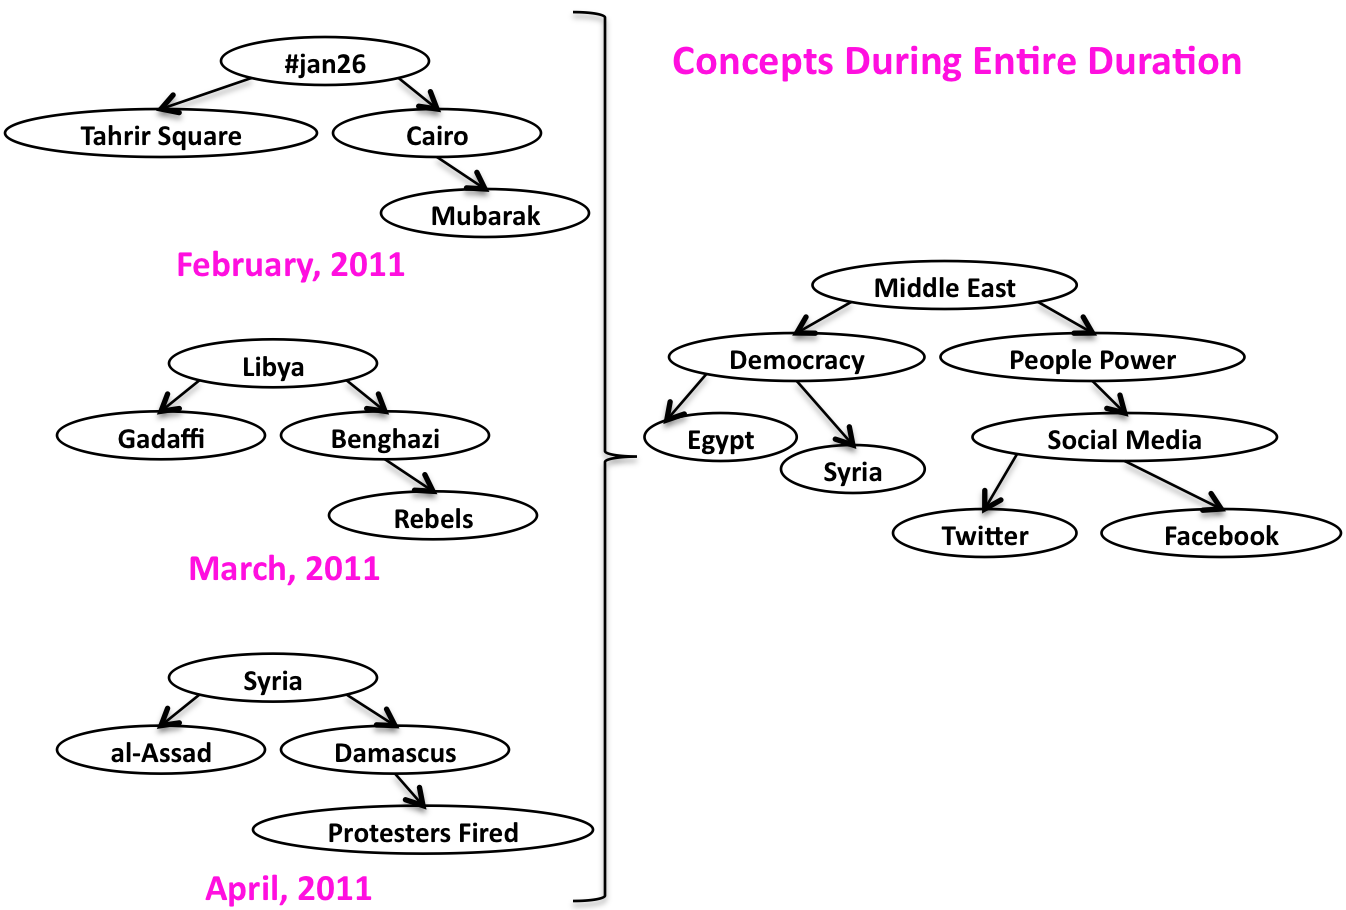
\includegraphics[width=3.0in]{images/concept_examples}
\caption{Examples of concept hierarchies during Middle-East revolutions in 2011.}
\label{fig:concept-examples}
\end{center}
\end{figure}

\section{Problem Statement}
\medskip Before describing the challenges in our problem, we first describe some general properties of algorithms that are designed for social media related information streams \cite{joao:2010:kdd}: 

\smallskip\noindent\textbf{Property 1}: As large amounts of data is generated in data streams at a very high rate, it is unrealistic to keep entire stream in main memory or even secondary storage during analysis. Hence, these algorithms should be single-pass algorithms that use approximation techniques like sampling, randomization, Fourier transforms etc., to summarize information flowing in streams.

\smallskip\noindent\textbf{Property 2}: The results from stream analysis should be available in real-time. Hence, these algorithms should have the ability to process collected information quickly to generate results.  

\smallskip\noindent \textbf{Property 3}: Unlike general streams, streams in social media are highly susceptible to concept drift. In addition, the properties of streams also follow temporal and event driven patterns. Hence, algorithms developed for these streams should also be robust against changes occurring in streams.

\medskip With these properties in mind, we describe the challenges for topic hierarchy extraction from information streams: 
\begin{itemize}
\item The first challenge is to identify phrases that can be used to build a concept hierarchy. The simplest approach is to use all the phrases that appear in the stream. But, this approach is not scalable for information streams. Hence, we sample only trending phrases from the stream to discover concept hierarchies (Property 1). 
\item The next challenge is to identify trending phrases from a stream.  One approach, is to think of this problem as a version of frequent items problem, where the item score decays with time, and select top-k items as trending phrases. But, this approach neither guarantees that the top-k phrases returned are all trending, nor that all trending phrases are returned. In addition, the value of k is hard to set and does not depending on the dynamic stream properties. The details of this are given in Section~\ref{sec:related_work}. Hence, we propose an approach that identifies all the trending phrases in a stream and is flexible to the changing stream properties (Property 3).
\item Now to determine the properties of information streams that impacts discovery of trending phrases. In this paper, we identify these properties and show how values for these properties can be calculated empirically for an information stream.
\item The next challenge is to make sure the algorithm we discover is efficient  (Property 2).. The efficiency of our approach can be split into 2 parts: (i) Efficiency during trend discovery and (ii) Efficiency of concept hierarchy discovered. It is important that our algorithm is efficient and has the ability to generate real-time results (Property 2). We describe our approach to improve the efficiency of our algorithm in Section~\ref{sec:trending-phrase-graphs} and show the performance in Section~\ ref{sec:experiments}. We then compare the concept discovery time and quality of concepts discovered by our approach with the approach used in \cite{Sanderson:1999:derivingconcept} in Section~\ref{sec:experiments}
\end{itemize}

\section{Related Work}
In the problem of determining aggregates on data streams, which is made up of objects ordered in time, the challenge is to maintain statistics like count, mean, etc., about the objects in the stream. Our problem of finding trending phrases is closely related to a problem in this domain called frequent items (FI) finding problem. In FI problem, a data structure maintains the score of objects seen on the stream, using which we can determine top-k items. To be more accurate, our problem is related to an variant of FI problem called time-decayed FI problem, where recent objects have higher scores than the older ones. 

Cormode and Hadjieleftheriou in \cite{Cormode:2010:fi_survey} give details of several algorithms that have been proposed for FI problem. Based on \cite{Cormode:2010:fi_survey}, the solutions to FI problem can be split into counter-based algorithms \cite{Misra:1982:fi, Manku:2002:fi, Metwally:2005:fi}, quantile algorithms \cite{Greenwald:2001:fi, Shrivastava:2004:fi} and sketches \cite{Charikar:2002:fi}.  One approach that has been proposed to deal with the time-decayed FI problem is using a sliding window \cite{Datar:2002:fi, Arasu:2004:fi, Lee:2006:fi}. In these algorithms, the data structure maintains information for only last $n$ items or $n$ items during the past $t$ time units. One of the issues with this approach is the need to maintain extra space for older windows. The performance of the algorithm is dependent on the length of sliding window. To overcome these issues an approach that uses  exponentially decayed weights of items has been proposed by Cormode et. al. \cite{Cormode:2008:fi}. They show the performance of their algorithm using decay is close the algorithms that don't use decay.

Many of these algorithms use a data structure of fixed size $k$, that is updated during processing of the stream. When the data structure is full, an item is removed from it using some criterion and the newly observed item is added. Using a fixed size data structure of size $k$ has the advantage of not having to deal with problems associated with memory space. But, the dis-advantage of this approach is that the performance of an algorithm is highly dependent on $k$, which might not be easy to determine. A way to overcome the limitations imposed by a fixed-size data structure is to have an additional pruning step, that remove old elements using some heuristics. In our problem we are not interested in finding top-k elements but determining trending phrases which might be larger or smaller than a constant $k$, depending on the nature of stream at that time.  Hence, we will be using
an approach that uses decaying phrase scores with the additional step of pruning.

\section{Materials and Methods}
\begin{figure}
\begin{center}
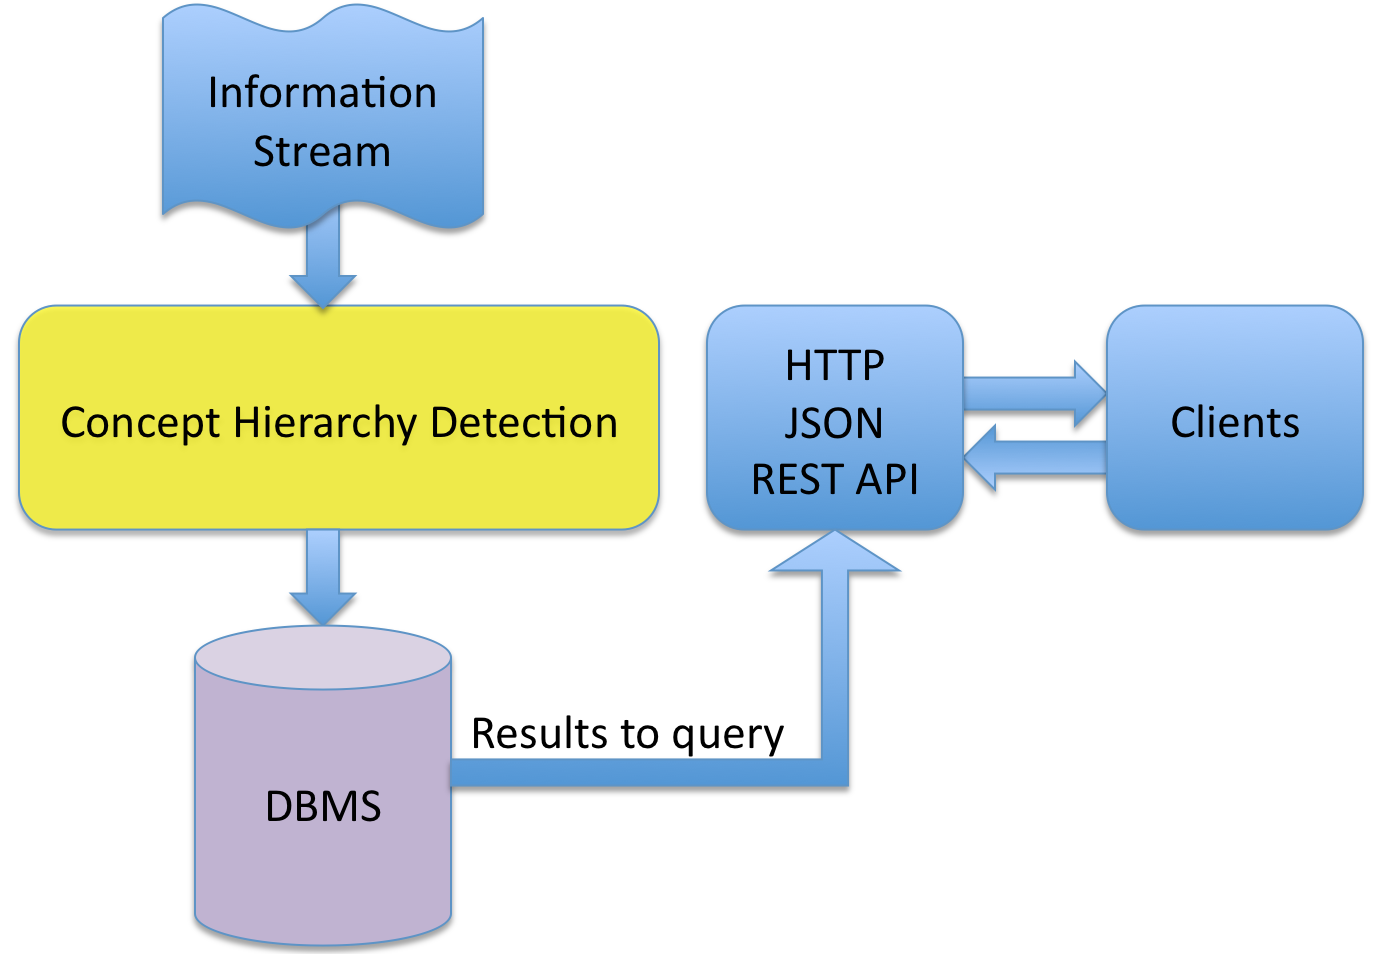
\includegraphics[width=3.0in]{images/architecture}
\caption{Architecture for Topic Detection from Information Streams.}
\label{fig:architecture}
\end{center}
\end{figure}

The architecture for topic detection from information streams is shown in Figure~\ref{fig:architecture}. The concept hierarchy detection module takes the information stream as input. The topic hierarchies obtained from the module is saved in a DBMS. We then develop a HTTP JSON REST API that provides an interface for clients to access the topic hierarchies discovered by the module. The API interacts with DBMS to retrieve information requested by clients. We now present the details of concept hierarchy detection module next.

\begin{figure*}[!t]
\begin{center}
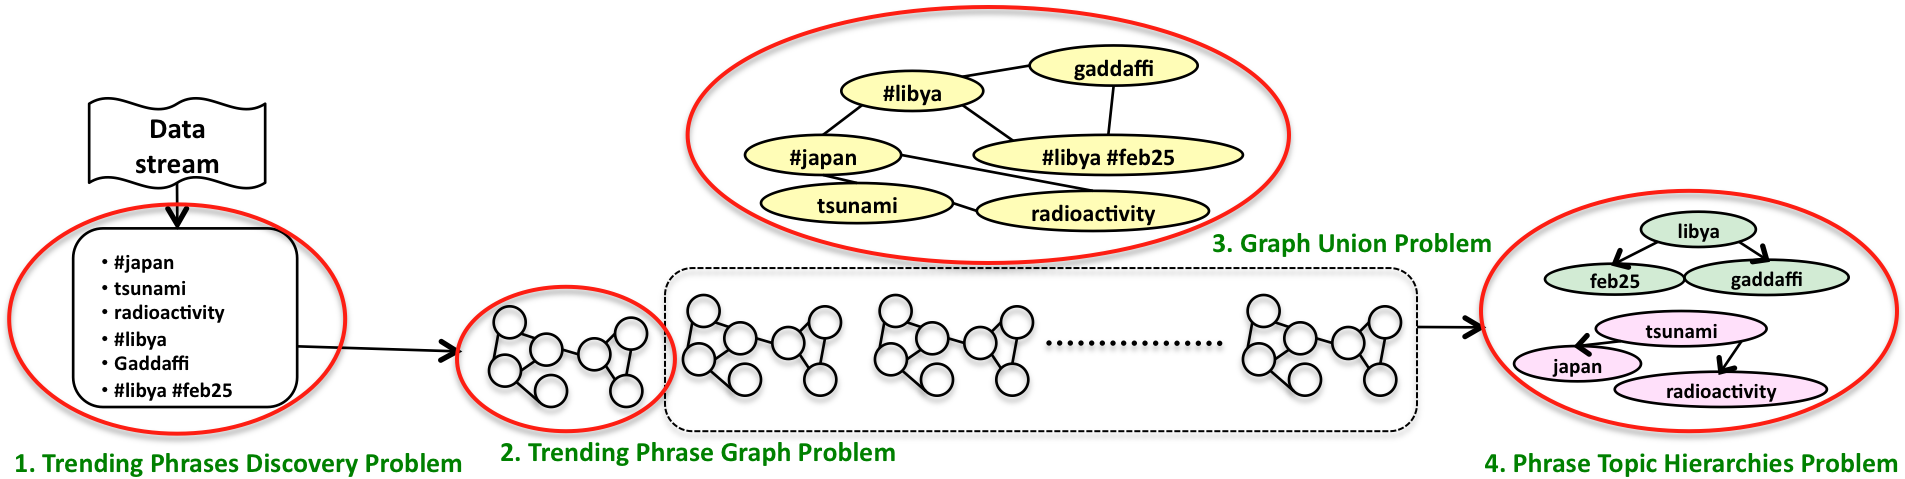
\includegraphics[width=7in]{images/introduction}
\caption{Problem description.}
\label{fig:introduction}
\end{center}
\end{figure*}

As shown in Figure~\ref{fig:introduction}, the problem of concept hierarchy detection can be broken into 4 sub-problems: (i) Trending Phrases Discovery Problem: This problem helps us determine phrases (concepts) that are trending in the stream. (ii) Trending Phrase Graph Problem: Given trending phrases at any-time, this problem helps us to determine relationships between various trending phrases. Representing related trending phrases as graph allows us to group together concepts related to a specific event and hence discover the event. (iii) Graph Union Problem: This problem helps us determine events and driving concepts using trending phrase graphs at different time-scales and at different granularities. (iv) Phrase Topic Hierarchies Problem: This helps us take a trending phrase graph and determine various events in it and the concepts that are driving the event in that graph.

The proposal is organized as follows. In Section~\ref{sec:trending-phrase-graphs} we work on the first two problems related to determining trending phrases and developing relationships among the trending phrases. We then describe the next two problems of combining trending phrase graphs at different time-scales and identifying topic hierarchies in them in Section~\ref{sec:phrase-hierarchy-retrieval}. We then describe our dataset and some experiments to evaluate our methods in Section~\ref{sec:experiments}.

\section{Trending Phrase Graph}
\label{sec:trending-phrase-graphs}
%\begin{center}
%\begin{tabular}{| c | c | p{1.75in}|}
%\hline
% \textbf{Type} &  \textbf{Symbol} &  \textbf{Description} \\ \hline
%\multirow{2}{*}{Data stream}
%	 & $D$ & Document stream \\  
%	 & $\eta$ & Stream phrase rate \\ \hline
%\multirow{6}{0.5in}{Candidate phrases}
%	 & $C$ & Set of candidate phrases \\
%	 & $T_{cp}$ & Candidate set pruning frequency \\ 
%	 & $S$ & Phrase score function \\ 
%	 & $\lambda_{c}$ & Candidate phrase score decay rate \\
%	 & $S_{t}$ & Trending constant \\
%	 & $S_{p}$ & Pruning constant \\\hline
%\multirow{5}{0.5in}{Phrase graph} 
%    	 & $\Gamma$ & Set of latest trending phrases \\ 
%    	 & $T_\gamma$ & Trend generation frequency \\ 
%    	 & $G_\gamma$ & Trending phrases graph \\ 
%    	 & $W_\gamma$ & Weight of edges in $G_\gamma$ \\
%    	 & $\lambda_\gamma$ & Edge weight decay rate in $G_\gamma$ \\ 
%\hline
%\end{tabular}
%\end{center}

%In this section, we describe our approach to discover trending phrases from a document stream. Challenges associated with sterams. desired properties in our algorithm like able to change with stream speed, meet challenges of stream etc.
%
%To solve this problem, we use an approach that is similar to the methods used in density-based clustering \cite{Chen:2007:density}. 


\subsection{Basic Definitions}

\begin{definition}
(\textbf{Data Stream}) A data stream $D = \{(d_1,\\ t_1), (d_2, t_1), (d_3, t_2) \dots \}$ is an ordered set of document tuples. The stream $D$ is of infinite size and is ordered in a non-decreasing fashion by time-stamp values of the documents. Note that, there might be multiple documents in the stream that share the same time-stamp.
\end{definition}

Examples of data streams that satisfy this property are tweets, blogs, mobile short messages, etc.

\begin{definition} 
(\textbf{Candidate Phrase}) Consider a document $d \in D$, where $|d|$ equal to the number of terms in the document. Let, $P_k$ be a set of phrases of length $k$. Then, $d$ can be represented using the set of phrases $P = P_1 \cup P_2 \cup \dots \cup P_{|d|}$. Such a phrase $p \in P$ is called a candidate phrase and the set of all the candidate phrases, observed in the data stream till time $t$, is represented as $C_t$.
\end{definition}

For example, the document ``Packers win Superbowl'' can be represented by P = \{``packers'', ``win'', ``superbowl'', ``packers win'', ``win superbowl'', ``packers win superbowl''\}. The phrases ``superbowl'', ``packers win'', etc are examples of candidate phrases and $P \subseteq C$.

\begin{definition} 
(\textbf{Candidate Phrase Instance}) A single candidate phrase $p$ may appear multiple times  in the stream. Each such instance of the phrase $p_i$ is called candidate phrase instance.
\end{definition}

For example, consider the document tuples (``Packers win'', $t_1$) and (``Champions packers '', $t_2$). In this case, the candidate phrase ``packers'' has two instances each with time-stamp $t_1$ and $t_2$ respectively. Similarly, ``win'' and ``champions'' have single instances.

\medskip Every candidate phrase instance $p_i$ is associated with a score, that decreases as the phrase ages, and a time-stamp $t_i$ of the document in which the instance was observed. The score $S(p_i, t)$ for $p_i$ at time t is given by:
\begin{align}
S(p_i, t) =  \lambda_c^{t-t_i} 
\label{eq:instance_score}
\end{align}
\noindent where $\lambda_c \in (0,1)$ is a constant know as \textbf{\textit{phrase score decay rate}}. 

\begin{definition} 
(\textbf{Candidate Phrase Scores}) In a stream we can observe several instances of a candidate phrase $p$. Let, $E(p, t)$ be the set of all the instances of $p$ that have been observed until time $t$. Then, the candidate phrase score at $t$, $S(p, t)$ is defined as the sum of all the candidate phrase instances of $P$.
\begin{align*}
S(p, t) &= \sum_{p_i \in E(p, t)} S(p_i, t)   =  \sum_{p_i \in E(p, t)}  \lambda_c^{t-t_i} 
\end{align*}
\end{definition}


The definition of $S(p, t)$ requires us to remember all the previous observed instances $E(p, t)$ for $p$ and its calculation taken O($|E(p, t)|$) time. This is in-efficient in real-world system where the number of phrases will be very large. Hence, we prove a proposition that will help us calculate this score efficiently in O(1) time and does not have the requirement of storing $E(p, t)$ .

\begin{proposition} 
Given a candidate phrase $p$ with score $S(p, t_l)$ at time $t_l$, if a phrase instance $p_i$ for $p$ is observed at time $t_n$, where $t_n>t_l$ then the new score for $p$ at $t_n$, $S(p, t_n)$  is given as:
\begin{align*}
S(p, t_n) =  \lambda_c ^{t_{n}-t_{l}} S(p, t_l) + 1
\end{align*}
\label{pro:candidate-phrase-score}
\end{proposition}
\begin{proof}
Let $P = \{p_1, p_2, \dots p_m\}$ be the set all the instance of the candidate phrases that have been observed till $t_n$. Hence,
\begin{align*}
S(p, t_l) &= \sum_{p_i \in P} S(p_i, t_l)
\end{align*}
\noindent Using (\ref{eq:instance_score}),  $\forall p_i \in P$ we can write:
\begin{align*}
S(p_i, t_n) &=  \lambda_c ^{t_{n}-t_{i}} = \lambda_c ^{(t_{n}-t_l) + (t_l - t_i) } = \lambda_c ^{(t_{n}-t_l)} \lambda_c ^{(t_l - t_i)} \\
S(p_i, t_n) &=\lambda_c ^{(t_{n}-t_l)}S(p_i, t_l)
\end{align*}
\noindent where $t_i$ is the time-stamp of $p_i$.\\

\noindent Using this we can write,
\begin{align*}
S(p, t_n) &= \sum_{p_i \in P} S(p_i, t_n) + 1  =  \sum_{p_i \in P} \lambda_c ^{(t_{n}-t_l)}S(p_i, t_l) + 1 \\
S(p, t_n) &=  \lambda_c ^{(t_{n}-t_l)}  \sum_{p_i \in P} S(p_i, t_l) + 1 =  \lambda_c ^{(t_{n}-t_l)} S(p, t_l) + 1
\end{align*}
\end{proof}

\subsection{Trending Phrases Discovery Problem}
\label{sec:trend:discovery:problem}
\begin{problem}
(\textbf{Trending Phrases Discovery Problem}) Given an infinite data stream $D$  and the set of candidate phrases $C_t$ observed in $D$, the trending phrases discovery problem is to identify the subset of phrases $\Gamma_t \subseteq C_t$ that are trending at time $t$.
\end{problem}

We can solve the trending phrases discovery problem, by defining a method to verify if a candidate phrase $p$ is popular or not. We can use the candidate phrase scores, discussed in the previous section, and \textit{\textbf{trending threshold $\theta_{tt}$} } to determine the popularity of $p$. Hence, for time $t$ we have:
\begin{align}
 \Gamma_t = \{p\ |\ S(p, t) \geq \theta_{tt}  \forall p \in C_t\} 
\label{eq:gamma}
\end{align}
\noindent Note that the value of $\theta_{tt}$  is dependent on the number of candidate phrases in $C_t$. This is done so that the discovery of trending phrases can adjust to temporal changes in the data stream.

\begin{figure}[!t]
\begin{center}
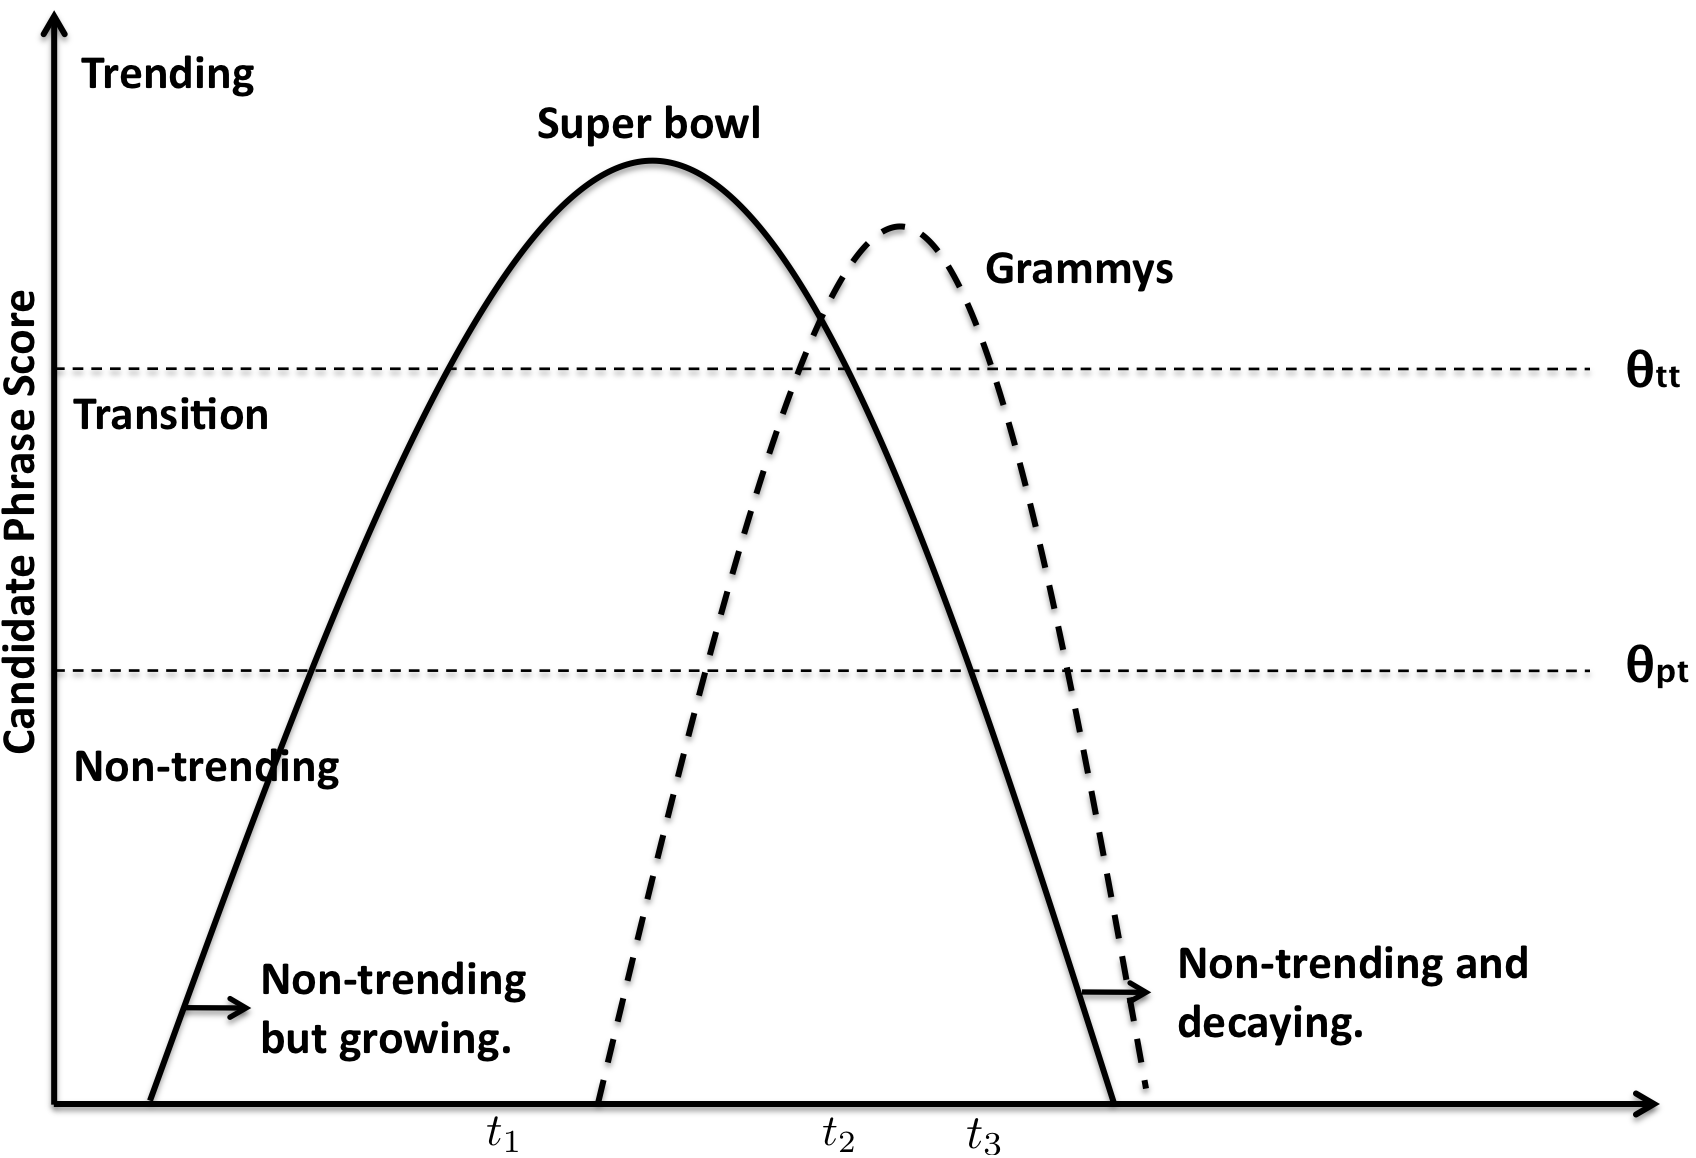
\includegraphics[width=3.0in]{images/candidate_phrases}
\caption{Examples for trending phrases discovery problem.}
\label{fig:candidate_phrases}
\end{center}
\end{figure}

To understand this approach take a look at the example shown in Figure~\ref{fig:candidate_phrases}. It shows variation in scores for two candidate phrases ``super bowl'' and ``Grammys'' with time. To keep the example simple we assume that the phrase rate in the data stream doesn't change and hence value of $\theta_{tt}$ is unchanged. So, using (\ref{eq:gamma}) we have, $\Gamma_{t_1} = \{$``super bowl''$\}$, $\Gamma_{t_2} = \{$``super bowl'', ``Grammys''$\}$ and $\Gamma_{t_3} = \{$``Grammys'$\}$.

\medskip\noindent\textbf{Pruning Candidate Phrases}: In real-world applications, the size of candidate phrases $C_t$ becomes very large. This makes the determination of $\Gamma$ using (\ref{eq:gamma}) in-efficient. Hence, we describe a method to determine a set of candidate phrases to prune, $C_{t}'$ using \textit{\textbf{pruning threshold $\theta_{pt}$} }, where $C_{t}' \subseteq C_t$.  Like trending threshold, pruning threshold is also dependent on $C_t$.

Using the candidate phrase score, the two thresholds $\theta_{tt}$ and $\theta_{pt}$, split $C_t$ into 3 sets: trending, transitional and non-trending. An example of this is shown in Figure~\ref{fig:candidate_phrases}. Though the  candidate phrases to prune are in the non-trending set, not all the phrases in this set can be pruned. This is because, the candidate phrases that are in non-trending set can be either be trending up or trending down.  Figure~\ref{fig:candidate_phrases} shows both the cases for the phrase ``Super bowl''. The phrases to be pruned are the ones that are trending down, but we cannot determine the direction of the trend just based on the candidate phrase score. Hence, we will the using some heuristic approaches to prune the candidate phrases.

For a candidate phrase $p \in C_t$ that is in the non-trending set we use the last time a phrase instance of $p$ was observed, $t_p$ to decide if it should be pruned.  To  determine $C_{t}'$, we propose two approaches that use $t_p$:  (i) deterministic approach (ii) randomized approach. 
These approaches also use a parameter \textit{\textbf{maximum phrase inactivity time $T_{pi}$}}.

\medskip Using the deterministic approach $C'$ is defined as follows:
\begin{align}
C_{t}' =  \{p\ |\ S(p, t) \leq \theta_{pt} \ and\ (t - t_p) \geq T_{pi}\    \forall p \in C_t\} 
\label{eq:deterministic-prune}
\end{align}

The randomized approach uses a function $R(p, t)\  \forall p \in C_t$ defined as:
\[
  R(p, t) = \left\{ 
  \begin{array}{l l}
    0 & \quad \text{if $t-t_p < T_{pi}$}\\
    1 & \quad \text{if $t-t_p \geq 2T_{pi}$}\\
   coinFlip(\frac{t-t_p}{2T_{pi}}) & \quad \text{Otherwise}\\
  \end{array} \right.
\]

\noindent where, $coinFlip: [0, 1] \rightarrow \{0, 1\} $, is a function where the probability of 1 increases as input is closer to 1. Now, $C_{t}'$ is defined as follows:
\begin{align}
C_{t}' =  \{p\ |\ S(p, t) \leq \theta_{pt} \ and\ R(p, t)=1 \    \forall p \in C_t\} 
\label{eq:randomized-prune}
\end{align}

\subsection{Trend Threshold Parameters} 
In the previous section we described how $\theta_{tt}$ and $\theta_{pt}$ can be used to determine $\Gamma$ efficiently. In this section, we describe methods to calculate these threshold parameters using data stream properties.

We first give a lemma that gives us the upper bound on the sum of scores for all the candidate phrase instances that have been observed on the data stream. We will then use the lemma to show the theorem that determines the thresholds. The proofs have been left out of this proposal.

\begin{lemma}
Given a data stream $D$ with a phrase rate of $\eta$ and the set of all candidate phrase instances $P_t$ that have been observed on $D$ during time intervals $0,1,2... t$, we have:
\begin{align*}
\sum_{p_i \in P_t}S(p_i, t) \leq \frac{\eta}{1-\lambda_c} \hspace{0.07in} \text{ and } \hspace{0.07in} \
\lim_{t \rightarrow \infty}{\sum_{p_i \in P_t}S(p_i, t)} = \frac{\eta}{1-\lambda_c}
\end{align*}
\label{cor:threshold}
\end{lemma}
%\begin{proof}
%For any time $t$, $ \sum_{p_i \in P_t}S(p_i, t)$ is the sum of scores for all the candidate phrase instances that have been observed on $D$ in [0, t] time intervals. 
%
%Using  (\ref{eq:instance_score}) for an instance $p_i$, we can write:
%\begin{align*}
%\sum_{p_i \in P_t}S(p_i, t) = \sum_{p_i \in P_t} \lambda_c^{t-t_i}
%\end{align*}
%where $t_i \in [0, t]$, is the time interval $p_i$ was observed in the stream.
%
%Note that, by our definition of $D$  there could be multiple phrase instances with the same value for $t_i$. The number of phrase instances every interval is given by $\eta$. Hence, we have,  
%\begin{align*}
%\sum_{p_i \in P_t}S(p_i, t) &= \eta\  (\lambda_c^{t-t_0} + \lambda_c^{t-t_1} + \dots + \lambda_c^{t-t}) \\
%&= \eta\  \left(\frac{1-\lambda_{c}^{t+1}}{1-\lambda_c}\right) \\
%\sum_{p_i \in P_t}S(p_i, t)  &\leq \frac{\eta}{1-\lambda_c}
%\end{align*}
%By, taking $\lim_{t \rightarrow \infty}$ on either sides, we have:
%\begin{align*}
%\lim_{t \rightarrow \infty} {\sum_{p_i \in P_t}S(p_i, t)}  = \lim_{t \rightarrow \infty} {\eta\   \left(\frac{1-\lambda_{c}^{t+1}}{1-\lambda_c}\right)} = \frac{\eta}{1-\lambda_c}
%\end{align*}
%\end{proof}

\begin{theorem}
Given a data stream $D$ at a phrase rate $\eta$ and the set of candidate phrases $C_t$ at time $t$, the trending threshold $\theta_{tt}$ and the pruning threshold $\theta_{pt}$ are given as:
\begin{align*}
\theta_{tt} = \frac{\eta S_t}{|C_t|(1-\lambda_c)} \hspace{0.2in} \text{ and } \hspace{0.2in} \theta_{pt} = \frac{\eta S_p}{|C_t|(1-\lambda_c)}
\end{align*}
where, $S_t > 1$ and $S_p < S_t$ are data stream specific constants.
\label{the:threshold}
\end{theorem}
%\begin{proof}
%Lemma~\ref{cor:threshold}, gave us a upper limit for the sum of scores for all the candidate phrase instances. We can use this to determine the upper bound for average candidate phrase scores. The sum of candidate phrase scores, at time $t$, is given by $\sum_{p \in C_t} S(p, t)$, hence we have:
%\begin{align}
%\sum_{p \in C_t} S(p, t) = \sum_{p \in C_t} \sum_{p_i \in P_{tp}} S(p_i, t)
%\label{eq:theorem1}
%\end{align}
%where, for a candidate phrase $p \in C_t$, $P_{pt}$ is the set of all the candidate phrase instances of $p$ that have been observed in the time interval $[0, t]$ on $D$. So, for the set of all candidate phrase instances $P_t$ (Lemma~\ref{cor:threshold}), we can write $P_t = \cup_{p \in C_t} P_{pt}$. Now, using (\ref{eq:theorem1}):
%\begin{align*}
%\sum_{p \in C_t} S(p, t) &= \sum_{p_i \in P_{t}} S(p_i, t)\\
%\sum_{p \in C_t} S(p, t) &\leq \frac{\eta}{1-\lambda_c} \hspace{0.5in} [\because Lemma~\ref{cor:threshold}]
%\end{align*}
%Let $Avg_{C_t}$ be the average of candidate phrase scores for phrases in  $C_t$, then $Avg_{C_t}  = \frac{\sum_{p \in C_t} S(p, t)}{|C_t|}$
%\begin{align*}
%Avg_{C_t} &\leq \frac{\eta}{|C_t|(1-\lambda_c)} 
%\end{align*}
%We have now determined the upper-bound for $Avg_{C_t}$. Depending on the percentage of $C_t$ phrases we consider to be trending and the data stream properties we can select a constant $S_t > 1$, such that all candidate phrases with score greater than or equal to $Avg_{C_t}S_t $ can be considered trending. Thus by definition of trending threshold $\theta_{tt}$, we have:
%\begin{align*}
%\theta_{tt} = \frac{\eta S_t}{|C_t|(1-\lambda_c)}
%\end{align*}
%Similarly, depending on the percentage of $C_t$ phrases we consider to be non-trending and the data stream properties we can select a constant $S_p < S_t$,  such that all candidate phrases with score lesser than or equal to $Avg_{C_t}S_l $ can be considered non-trending. Thus by definition of pruning threshold $\theta_{pt}$, we have:
%\begin{align*}
%\theta_{pt} = \frac{\eta S_p}{|C_t|(1-\lambda_c)}
%\end{align*}
% \end{proof}

The values of $S_t$ and $S_p$ are still unknown and depend on the data stream and the application requirements. We, will describe methods to estimate these values in Section~\ref{sec:experiments} .


\subsection{Trending Phrase Graph Problem}
\begin{problem} (\textbf{Trending Phrase Graph Problem})
Given data stream $D$ and the set of latest trending phrases $\Gamma$, construct an un-directed graph $G_{\gamma t}(V, E)$  that describes the relationships between trending phrases at time $t$, such that $V = \Gamma$ and the edge weight $w(u, v)\ \forall\ u, v \in V$, measures closeness between the phrases $u$ and $v$.
\end{problem}

We use two features to measure the closeness (edge-weights) between phrases: 
\begin{itemize}
\item \textbf{Co-occurance}:  Phrases that appear together more often should be closer to each other than phrases that don't appear together. This feature helps in formation of clusters of related phrases which will be used in topic hierarchy detection.
\item \textbf{Temporal locality}: Phrases co-occurring in recent time intervals should be closer to each other than the phrases that have co-occurred in previous time intervals. This feature helps us to model dynamics of topic evolution like introduction of new phrases into an existing topic cluster and removal of older phrases, topic split, topic merge etc.
\end{itemize}

Consider phrases $u$ and $v$, that last co-occurred at $t_l$ and have edge weight  $w_{t_l}(u, v)$. When these phrases co-occur again at time $t_n$, we calculate the new edge weight as:
\begin{align}
w_{t_n}(u, v) = w_{t_l}(u, v)\lambda_{\gamma}^{t_n-t_l  } + 1  
\label{eq:phrase-graph-edge-weight}
\end{align}
\noindent where $\lambda_{\gamma} \in [0, 1]$ is a constant called phrase graph edge decay rate. To model temporal locality, that we described earlier, we decay the edge weights in phrase graph using (\ref{eq:phrase-graph-edge-weight}).


\subsection{Trending Phrase Graph Algorithm}

In this section, we describe the trending phrase graph algorithm that we have developed based on the analysis in the previous sections. The complete algorithm is given in Algorithm~\ref{alg:trending-phrase-algorithm}.

\algsetup{indent=2em}
\newcommand{\TrendPhrasesDiscovery}{\ensuremath{\mbox{\sc TrendPhrasesDiscovery}}}
\begin{algorithm}[t]
\caption{$\TrendPhrasesDiscovery$}
\begin{algorithmic}
\STATE \textbf{Initiliaize:}  $\Gamma = \emptyset$
\WHILE{True}
\STATE \textbf{1. Process document $d_i$:} Get the next document $d_i$, generated at $t_i$, from the input data stream. Extract phrases $P_i$ from the document.
\STATE \textbf{2. Update $C_{t_i}$:} Update the score of every phrase $p \in P_i$, where $t_p$ is the time the last time $p$ was updated, using:
\begin{align*}
S(p, t_i) =  \lambda_c ^{t_{i}-t_{p}} S(p, t_p) + 1 \hspace{0.4in}[\because Proposition~\ref{pro:candidate-phrase-score}]
\end{align*}
\STATE \textbf{3. Update $G_{\gamma t_i}$:} For every pair of phrases in $ \{ (u, v) | \forall\ u,v \in P_i \cap \Gamma\}$, if an edge exists between $u$ and $v$ update it using (\ref{eq:phrase-graph-edge-weight}). If an edge does not exist add and edge with $w_{t_i}(u, v) = 1$.
\STATE  \textbf{4. Prune $C_{t_i}$:} Every $T_{cp}$ time intervals, prune $C_{t_i}$. Before pruning, for every phrase $p \in C_{t_i}$ update its candidate phrase score using:
\begin{align*}
S(p, t_i) =  \lambda_c ^{t_{i}-t_{p}} S(p, t_p) 
\end{align*}
Now, prune $C_{t_i}$ using either Equation~\ref{eq:deterministic-prune} or Equation~\ref{eq:randomized-prune}.
\STATE \textbf{5. Update $\Gamma$:} Every $T_\gamma$ time intervals, re-generate the set of trending phrases $\Gamma_{t_i}$ from $C_{t_i}$. Initialize $\Gamma_{t_i}$ to $\emptyset$ and for every phrase $p \in C_{t_i}$ update its candidate phrase score using:
\begin{align*}
S(p, t_i) =  \lambda_c ^{t_{i}-t_{p}} S(p, t_p) 
\end{align*}
Now, re-generate $\Gamma_{t_i}$ using Equation~\ref{eq:gamma}. Set $\Gamma = \Gamma_{t_i}$.\\
Also remove phrases from $G_{\gamma t_i}$ that are not present in $\Gamma$.
\ENDWHILE
\end{algorithmic}
\label{alg:trending-phrase-algorithm}
\end{algorithm}

The algorithm first initializes $\Gamma$ to an empty set. $\Gamma$ contains the set of latest trending phrases that are generated every $T_\gamma$ intervals. The algorithm operates on a single document during every iteration. For every document, it first retrieves the phrases in the document and updates the candidate phrase scores for each phrase. It also, updates the edges in $G_{\gamma {t_i}}$ for every pair of phrases that are trending. Every $T_{cp}$ time intervals $C_{t_i}$ is pruned as described in Section~\ref{sec:trend:discovery:problem}. Similarly, every $T_\gamma$ time intervals it generates the set of latest trending phrases $\Gamma$.

\section{Phrase Hierarchy Retrieval}
\label{sec:phrase-hierarchy-retrieval}
%In this section we give details of how to retrieve a collection o

\subsection{Graph Union Problem}
\begin{problem}(\textbf{Graph Union Problem})
For a data stream $D$, given a time interval $I = [t_l, t_u]$ and graph union threshold $\theta_u$, construct an un-directed graph $G_u(V_u, E_u)$ that describes the relationships between trending phrases during the entire interval I. The edge weights $w_u(u, v),\ \forall\ u, v \in V_u$ measures closeness between $u$ and $v$. Consider, $t_l$ and $t_u$ to be multiples of a constant $\delta$.
\end{problem}

In the interval $I$, $t_l$ and $t_u$ are multiples of $\delta$, hence, $I$ can be broken into $n =  \left( \lfloor \frac{t_u - t_l}{\delta} \rfloor + 1 \right)$ time intervals of equal length. For example, when $\delta = 1$, for the interval $[1,10]$, $n=10$; and for $[3,7]$, $n=5$. So, we generate the trend phrase graphs $G_\gamma$ at regular intervals of length $\delta$ and then combine the graphs using some method to construct $G_u$ for $I$. We can construct $G_u$ using two different approaches: (i) Linear graph union, which has a complexity of $O(n)$, (ii) Logarithmic graph union, which with moderate amount of preprocessing has a complexity of $O(\log_2{n})$

\algsetup{indent=2em}
\newcommand{\GraphUnion}{\ensuremath{\mbox{\sc GraphUnion}}}
\begin{algorithm}[t]
\caption{$\GraphUnion(G_u', I, \theta_u)$}
\begin{algorithmic}
%\STATE \textbf{1. Get $G_u'$:} Construct $G_u' = \{G_{\gamma t_i} |\ \forall\ t_i \in I \}$. 
%\STATE \textbf{2. Update  $G_u'$}: For every graph in $G_u'$, initialize the weights of every edge to $1$.
\STATE \textbf{1. Construct  $G_u(V_u, E_u)$}: Construct the union graph $G_u(V_u, E_u)$, such that:
\begin{align*}
V_u &= \cup_{G_{\gamma t_i} \in G_u'} V_{\gamma t_i} \\
E_u &= \cup_{G_{\gamma t_i} \in G_u'} E_{\gamma t_i}
\end{align*} 
For every pair of connected vertices $(v_1, v_2) \in V_u$, set $ W_u(v_1, v_2, I)$ to the sum of weights of all the parallel edges between $(v_1, v_2)$. Replace all the parallel edges with a single edge.
\STATE \textbf{2. Filter  $G_u(V_u, E_u)$}:  Remove any edge $(v_1, v_2) \in E_u$, that meets the condition:
 \begin{align*}
 W_u(v_1, v_2, I) < \theta_u \left( \lfloor\frac{t_u - t_l}{\delta}\rfloor + 1\right)
\end{align*} 
\end{algorithmic}
\label{alg:graph-union}
\end{algorithm}

\medskip\noindent\textbf{Generic Graph Union Algorithm}: We design an algorithm to determine the graph union $G_u$, given a set of graphs $G_u'$, from which it should be constructed. This algorithm will be used by both the linear and logarithmic graph union methods, described later in this section. The complete algorithm is given in Algorithm~\ref{alg:graph-union}. The algorithm takes graph set $G_u'$, interval $I$ and the threshold $\theta_u$ as input and constructs $G_u$.

In the first step of the algorithm, we combine all the vertices and edges in $G_u'$ to form $G_u$. For all vertices $(v_1, v_2) \in V_u$, the parallel edges in $G_u$ are then replaced by a single edge $(v_1, v_2)$ and the edge weight $ W_u(v_1, v_2, I)$ is set to the sum of parallel edges between $v_1$ and $v_2$. If there is a single edge between $(v_1, v_2)$ then $ W_u(v_1, v_2, I)$ is set to the weight of that edge. In a way, the value $ W_u(v_1, v_2, I)$ is equal to the number of times edge $(v_1, v_2)$ occurs in the interval $I$.

In the next step, we filter $G_u$ to remove edges that don't meet the graph union threshold criterion $\theta_u$. This threshold specifies the percentage of time intervals in which a edge must have existed. This corresponds to the number of times two trending phrases are related to each other in $I$. 

%\begin{lemma}
%Given two disjoint intervals $I_1$ and $I_2$, the following relationship holds:
%\begin{align*}
%W_u(v_1,v_2, I_1 \cup I_2) = W_u(v_1,v_2, I_1) +W_u(v_1,v_2, I_2)
%\end{align*}
%irrespective of the method (linear or logarithmic) used to determine $G_u$.
%\label{lemma:graph-union-weights}
%\end{lemma}
%\begin{proof}
%By definition $W_u(v_1,v_2, I)$, is equal to the number of times edge $(v_1, v_2)$ appears in interval $I$. Now, since $I_1$ and $I_2$ are disjoint, the number of times $(v_1, v_2)$ appears in $I_1 \cup I_2$ is equal to the number of times $(v_1, v_2)$ appears in both intervals $I_1$ and $I_2$.
%\end{proof}

\medskip\noindent\textbf{Linear Graph Union}: In this approach, we create the set of graphs $G_u'$ that contains all the $G_\gamma$ graphs for the interval $I$.  
\begin{align*}
G_u' &= \{G_{\gamma t_l}, G_{\gamma t_{l}+\delta}, G_{\gamma t_{l}+2\delta} , \dots , G_{\gamma t_{u}} \}\\
G_u' &= \{G_{\gamma t}\}_{t=t_l}^{t_u}
\end{align*} 
For every graph in $G_u'$, we set all the weight of all edges to $1$. With the modified, $G_u'$, graph union algorithm described in Algorithm~\ref{alg:graph-union} can be used to construct $G_u$. Since, $G_u'$ has a cardinality of $n$, the algorithm has a complexity of $O(n)$.

\medskip\noindent\textbf{Logarithmic Graph Union}: Like before, we generate a trend phrase graph $G_\gamma$ at every interval of length $\delta$. But, in addition to these graphs, we also generate extra graphs called combined trending phrase graphs $G_{\gamma}^k$ that are formed by combination of $k$ different $G_\gamma$ graphs. 

Combining information from smaller $G_\gamma$ graphs enables us to develop efficient algorithms for construction of $G_u$, with moderate amount of preprocessing during the generation of $G_\gamma$. $G_{\gamma}^k$ is constructed using graphs from $G_{\gamma t}^{k'}$, which consists of trending phrase graphs for the current interval and the past $k-1$ intervals, $G_{\gamma t}^{k'} = \{G_{\gamma (t-i\delta)}\}_{i=0}^{i=k-1}$. For example, when $\delta=1$, $G_{\gamma 4}^4$ is formed by combining graphs in $G_{\gamma 4}^{4'} = \{ G_{\gamma 4}, G_{\gamma 3}, G_{\gamma 2}, G_{\gamma 1} \}$. 
%\begin{align*}
%G_{\gamma t}^{k'} = \{G_{\gamma  t}, G_{\gamma (t-\delta)}, G_{\gamma (t-2\delta)}, \dots, G_{\gamma (t-(k-1)\delta)}\}
%\end{align*}

We generate $G_{\gamma t}^k$ using steps similar to that followed in linear graph union. We first set the weight of all edges in  all the graphs in $G_{\gamma t}^{k'}$ to $1$. We then combine the graphs as decribed in Step 1. of Algorithm~\ref{alg:graph-union}. But, we don't filter out any edges like we did in that case. Filtering of edges is done only during construction of $G_u$.

To build $G_u$ given an interval $I$, we have to first determine $G_u'$, the set of combined trending phrase graphs using which it will be constructed. For an interval $I=[a,b]$, the corresponding combined trending phrase graph is $G_{\gamma b} ^{b-a+1}$. So, we split $I$ into several intervals for which combined trending phrase graphs are pre-built. The algorithm to generate these intervals is trivial and a recursive algorithm to generate them is given in \cite{Dubinko:2006:tags}. For example to build $G_u$ for the interval $I = [1,7]$, we split $I$ into, $[1,4]$, $[5,6]$ and $[7,7]$, which gives $G_u' = \{G_{\gamma 4}^4, G_{\gamma 6}^2, G_{\gamma 7}^1\}$.

Untill now, we have described how to construct $G_u$ using $G_{\gamma t}^k$, and how to generate $G_{\gamma t}^k$. But, we haven't described when to generate $G_{\gamma t}^k$. We now describe this. In logarithmic graph union method, we construct extra graphs at different times. At any time $t$, where $t$ is even and a multiple of $\delta$, we generate $\log_2{t}+1$ additional graphs. The graphs generated are $\{G_{\gamma t}^{\frac{t}{2^i}}\}_{i=0}^{\log_2{t}}$. For example, when $t = 8$, we generated $4$ graphs: $G_{\gamma 8}^{8}$, $G_{\gamma 8}^{4}$, $G_{\gamma 8}^{2}$ and $G_{\gamma 8}^{1}$. 

%\begin{align*}
%G_{ug}' &= \{G_{\gamma t_l}^\delta, G_{\gamma t_{l+\delta}}^\delta, G_{\gamma t_{l+2\delta}}^\delta , \dots , G_{\gamma t_{u}}^\delta \} \\
%G_{ug}' &= \{G_{\gamma t}^\delta\}_{t=t_l}^{t_u}
%\end{align*}
\begin{figure}[!t]
\begin{center}
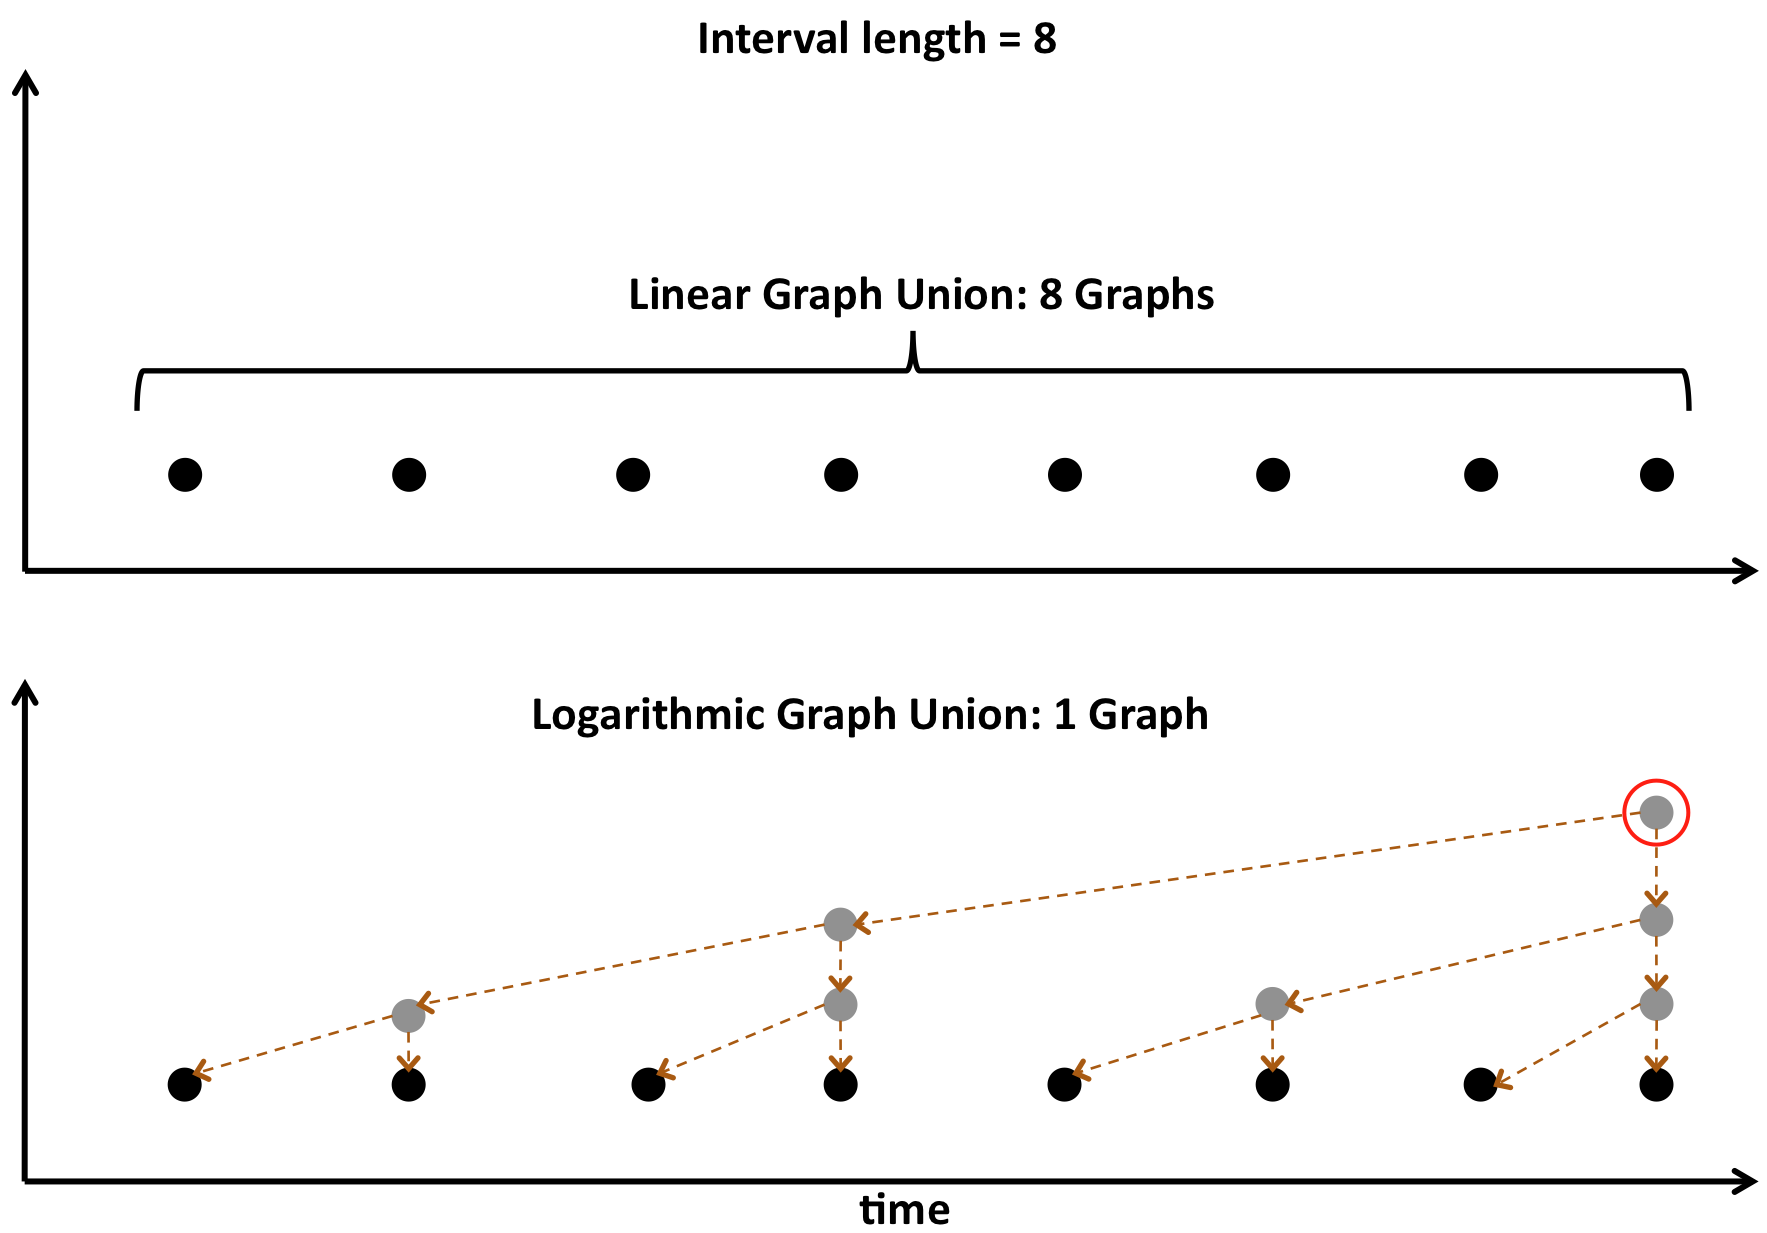
\includegraphics[width=3.0in]{images/graph_union_example}
\caption{Examples for graph union using linear and logarithmic methods.}
\label{fig:graph_union_example}
\end{center}
\end{figure}

\medskip An example, of graphs generated using these two different methods is shown in Figure~\ref{fig:graph_union_example}. We see that, for an interval of length $8\delta$, the linear graph union approach requires processing of 8 graphs, while logarithmic approach requires only $1$ graph.

\medskip We now give a definition of identical graphs and then give a theorem that shows the graphs generated by both these methods are identical.

\begin{definition} (\textbf{Identical Graphs})
Given an interval $I$ and a threshold $\theta_u$,  two graphs $G_{u1}$ and $G_{u2}$ constructed using the graph union methods, described before, are said to be identical iff the following conditions hold:
\begin{align*}
V_{u1} &= V_{u2} \text{, } E_{u1} = E_{u2} \text{, and}\\
W_{u1}(v_1, v_2, I) &=  W_{u2}(v_1, v_2, I)\ \forall\ (v_1, v_2) \in E_{u1}
\end{align*}
\end{definition}

\begin{theorem}
Given an interval $I$ and a threshold $\theta_u$, the graph generated by both, linear and logarithmic graph union methods are identical. 
\end{theorem}
%\begin{proof}
%Let the $G_{ul}$ and $G_{ug}$ be the graph generated using linear and logarithmic approach respectively. Let, $G_{ul}^{'}$  and $G_{ug}^{'}$ be the sets of trending phrase graphs used to construct $G_{ul}$ and $G_{ug}$ as described before. Then if the length of the interval $I = [t_l, t_u]$ we have:
%\begin{align*}
%G_{ul}' &= \{G_{\gamma t}\}_{t=t_l}^{t_u}
%\end{align*}
%In case of logarithmic approach, $I$ can be broken into several intervals of length $\delta$. For example, when $\delta =1$, interval $[1,4]$ can be recursively broken into intervals $\{[1,2], [2,3], [3,4]\}$. Hence, $G_{ug}'$ can be written as:
%\begin{align*}
%G_{ug}' &= \{G_{\gamma t}^\delta\}_{t=t_l}^{t_u}
%\end{align*}
%Now, we can show  $G_{ul}$ and $G_{ug}$  are identical be showing that graphs generated using  $G_{ul}^{'}$ and $G_{ug}^{'}$ are identical. We will use mathematical induction to prove this theorem.
%
%\medskip\noindent\textbf{Basis:} We first show that $G_{ul}$ and $G_{ug}$ are identical if $I = [t_l, t_l]$ is of length $\delta$.
%
%For linear method $G_{ul}' = \{G_{\gamma t_l} \}$. Since, there is only one graph in  $G_{ul}'$, using Algorithm~\ref{alg:graph-union}, we get $G_{ul}$, where:
%\begin{align*}
%V_{ul} &= V_{\gamma t_l} \text{, } E_{ul} = E_{\gamma t_l} \text{, and }\\
%W_{ul}(v_1, v_2, I) &=  1\ \forall\ (v_1, v_2) \in E_{ul} \tag{A}
%\end{align*}
%
%For logarithmic method $G_{ug}' = \{G_{\gamma t_l}^{\delta} \}$. As described in the method before, $G_{\gamma t_l}^{\delta} $ is the graph obtained after $G_{\gamma t_l}$ goes through Step $1$ of Algorithm~\ref{alg:graph-union} only. $G_{ug}$ is obtained after combining graphs in $G_{ug}' $ and filtering out edges below threshold. Thus we get $G_{ug}$, where:
%\begin{align*}
%V_{ug} &= V_{\gamma t_l} \text{, } E_{ug} = E_{\gamma t_l} \text{, and }\\
%W_{ug}(v_1, v_2, I) &=  1\ \forall\ (v_1, v_2) \in E_{ug} \tag{B}
%\end{align*}
%Using (A) and (B) we show that $G_{ul}$ and $G_{ug}$ are identical if $I \in [t_l, t_l]$ is of length $\delta$.
%
%\medskip\noindent\textbf{Inductive Step:} In this step we use the inductive hypothesis that $G_{ul}$ and $G_{ug}$ are identical if $I_n = [t_l, t_l+n\delta]$ is of length $n$, and have to show that $G_{ul}$ and $G_{ug}$ are identical for an interval $I_{n+1} = [t_l, t_l+(n+1)\delta]$ of length $n+1$.
%
%Let $I_x = [t_l+(n+1)\delta,\ t_l+(n+1)\delta ]$ be the $(n+1)^{th}$ interval, such that $I_{n+1} = I_n \cup I_x$.
%
%For linear method $G_{ul}' = \{G_{\gamma t}\}_{t=t_l}^{t_l+n\delta} \cup \{G_{\gamma t_l+(n+1)\delta}\}$. So, we have:
%\begin{align*}
%V_{ul} &= \cup_{t=t_l}^{t_l+n\delta} V_{\gamma t} \cup V_{\gamma t_l+(n+1)\delta} \tag{C} \\
%E_{ul} &=  \cup_{t=t_l}^{t_l+n\delta} E_{\gamma t} \cup E_{\gamma t_l+(n+1)\delta}\\
%W_{ul}(v_1, v_2, I_{n+1}) &=  W_{ul}(v_1, v_2, I_n) + 1\ \forall\ (v_1, v_2) \in E_{ul} 
%\end{align*}
%
%For logarithmic method $G_{ug}' = \{G_{\gamma t}^\delta\}_{t=t_l}^{t_l+n\delta} \cup \{G_{\gamma t_l+(n+1)\delta}^\delta\}$ So, we get:
%\begin{align*}
%V_{ug} &= \cup_{t=t_l}^{t_l+n\delta} V_{\gamma t}^\delta \cup V_{\gamma t_l+(n+1)\delta}^\delta \\
%E_{ug} &=  \cup_{t=t_l}^{t_l+n\delta} E_{\gamma t}^\delta \cup E_{\gamma t_l+(n+1)\delta}^\delta\\
%W_{ug}(v_1, v_2, I_{n+1}) &=  W_{ug}(v_1, v_2, I_n) + 1\ \forall\ (v_1, v_2) \in E_{ug} 
%\end{align*} 
%Using  inductive hypothesis and results from (A) and (B), we can write:
%\begin{align*}
%V_{ug} &= \cup_{t=t_l}^{t_l+n\delta} V_{\gamma t} \cup V_{\gamma t_l+(n+1)\delta} \tag{D} \\
%E_{ug} &=  \cup_{t=t_l}^{t_l+n\delta} E_{\gamma t} \cup E_{\gamma t_l+(n+1)\delta}\\
%W_{ug}(v_1, v_2, I_{n+1}) &=  W_{ul}(v_1, v_2, I_n) + 1\ \forall\ (v_1, v_2) \in E_{ul} 
%\end{align*}
%Using (C) and (D) we show that $G_{ul}$ and $G_{ug}$ are identical when interval is of length $n+1$.
%\end{proof}

\subsection{Phrase Topic Hierarchies Problem}
\label{sec:phrase-topic-hierarchy}
\begin{problem}(\textbf{Phrase Topic Hierarchies Problem})
Given an undirected graph $G(V, E)$ of trending phrases, construct phrase topic hierarchies $H$.
\end{problem}

We divide the task of determining topic hierarchies $H$ using $G$ into two steps. In the first step we cluster $G$ to determine topics. We then use the individual clusters to determine topic hierarchies. We next describe these two steps next. 

\medskip\noindent\textbf{Graph Clustering}: In trending phrases graph $G$, phrases related to each other are close to each other. Hence, we cluster this graph to determine topic clusters that are trending together. We use the Markov Cluster Algorithm (MCL) \cite{Dongen:2000:mcl}, to cluster $G$. MCL is a fast and scalable clustering algorithm that uses simulation of flows in the graph to cluster it. We then use each of these clusters to determine topic hierarchies.

\medskip\noindent\textbf{Topic Hierarchies}: A topic hierarchy is a directed acyclic graph, which contains phrases as vertices and the relationships between phrases is indicated using directed edges. For every topic cluster in $G$, we determine the \textbf{\textit{root phrase}} and then construct the hierarchy using breadth first traversal. The vertex to be selected as root phrase should describe the cluster well and hence should be a significant vertex based on some centrality measure. The metric we use to choose root phrase will determine the type of relationship the topic hierarchy describes. We describe two types of topic hierarchies and the metric that is used to generate these hierarchies:
\begin{itemize}
\item \textbf{Driven By Genrality}: In this method the topic hierarchy is built such that a parent node describes a concept that is more general than the child node. One way to define genrality of a node in a graph is to measure the number of nodes (degree centrality) it is connected to. For example, a node like ``Middle-East'' will be connected to more phrases in topic cluster about Middle-East than the node ``Hosni Mubarak''. Hence, we can say ``Middle-east'' is more general than ``Hosni Mubarak''.  
%To mea node that is asssociated with more nodes This is the simplest way of measuring the importance of a vertex in the cluster. The value of this measure is equal to degree of the vertex in the cluster. This measure can be useful because a trending phrase that is connected to several other phrases can be a good indicator of the topic of the cluster and would possibly be driving the topic. 
%\item \textbf{Betweenness Centrality}:  This metric measures the importance of a vertex based upon its ability to connect other vertices. A vertex which appears on many shortest paths for other vertices has a higher betweenness score. In terms of a cluster of trending phrases, a phrase with higher betweenness indicates that it is relevant in connecting different concepts in a topic and hence could be a driving topic.
\item \textbf{Driven By Popularity}: In Section~\ref{sec:trending-phrase-graphs}, we assigned scores to phrases, which were used in identifying trending phrases. We can use these scores to build a topic hierarchies such that a parent vertex has a trending score higher than the child vertex. For example, like before, consider the topic cluster about Middle-East, though ``Middle-East'' is connected to more vertices than ``Hosni Mubarak'', ``Hosni Mubarak'' might have a higher trend score than ``Middle-East''. This shows that ``Hosni Mubarak'' is in way driving the issues in Middle-East.
\end{itemize}
 
In this way, we can use two different metrics to construct phrase topic hierarchies, each giving us a different perspective of information on the real-time web.

\section{Evaluation}
\label{sec:experiments}
In this section, we describe the experimenents that we plan to conduct. The experiments are:
\begin{itemize}
\item \textbf{Stream Parameters Estimation}: In Section~\ref{sec:trending-phrase-graphs}, we described an algorithm to extract trending phrases from a data stream. The algorithm uses threshold parameters like trending threshold $\theta_{tt}$ and pruning threshold $\theta_{pt}$ which are dependent on data stream specific constants like $S_t$ and $S_p$ respectively. The algorithm also uses a parameter called stream parameter maximum phrase inactivity time $T_{pi}$, to improve its efficiency. We will propose methods to perform stream analysis to determine these parameters.
\item \textbf{Deterministic Vs Randomized Algorithm}: The trending algorithm can use deterministic or randomized depending on the approach taken to prune the candidate phrase set $C_t$. The approaches were described in Section~\ref{sec:trend:discovery:problem}. In this experiment, we will compare these two different approaches.
\item \textbf{Comparison with Sanderson's Approach}: We will compare our approach to generate topic hierarchies on a data stream with the approach used by Sanderson and Croft \cite{Sanderson:1999:derivingconcept}. 
\item \textbf{Examples of Topic Hierarchies}: We will finally show some examples of the concepts discovered using this approach.
\end{itemize}

We first describe details of the data streams that we will be using in our experiments.

\subsection{Data Streams For Evaluation}
\label{sec:data-stream}
To perform our experiments we will use data collected using Twitter Streaming API \footnote{dev.twitter.com}. We use two different streams: (i) Trending topic stream, and, (ii) Domain specific stream. To generate the trending topic stream, we get current trending topics using Twitter APIs  and use the ``track'' parameter of the filter method from Streaming API. To generate domain specific stream we first determine prominent users for $4$ domains - technology, entertainment, politics and sports, using snowball sampling approach described in \cite{Watts:2011:twitter}. Then for each domain we pick 1250 users and use the ``follow'' parameter of the filter method from Streaming API to generate domain specific stream. Some statistics from the streams is shown in Table~\ref{table:data-stream}. These statistics were calculated on a single day sample of these streams.

\begin{table}
 \begin{minipage}{5cm}
 \begin{center}
    \begin{tabular}{ c|c|c}
    \hline
    \textbf{Stream} & \textbf{Tweets\footnote{Every 5 minutes}} & \textbf{Phrase rate\footnote{Every minute}} \\ \hline\hline
    Trending topic stream & 3191.26  & 7714.04\\ \hline
    Domain specific stream & 87.54 & 382.90 \\ \hline
    \end{tabular}
    \end{center} 
      \end{minipage}
    \caption{Data stream properties}
  \label{table:data-stream}
 \end{table}
 
 \section{Conclusion}
 In this project, we proposed a framework for discovering, archiving and browsing topic hierarchies from information streams. We also presented the details of algorithms that can be used discover topic hierarchies from information streams. We finally gave the details of our dataset and evaluation methods we will be using to test the framework.


%\subsection{Stream Parameters Estimation}
%
% \begin{figure*}[ht]
%   \begin{center}
%     \subfigure[Scores by percentage]
%     {\label{fig:phrase-by-percentage}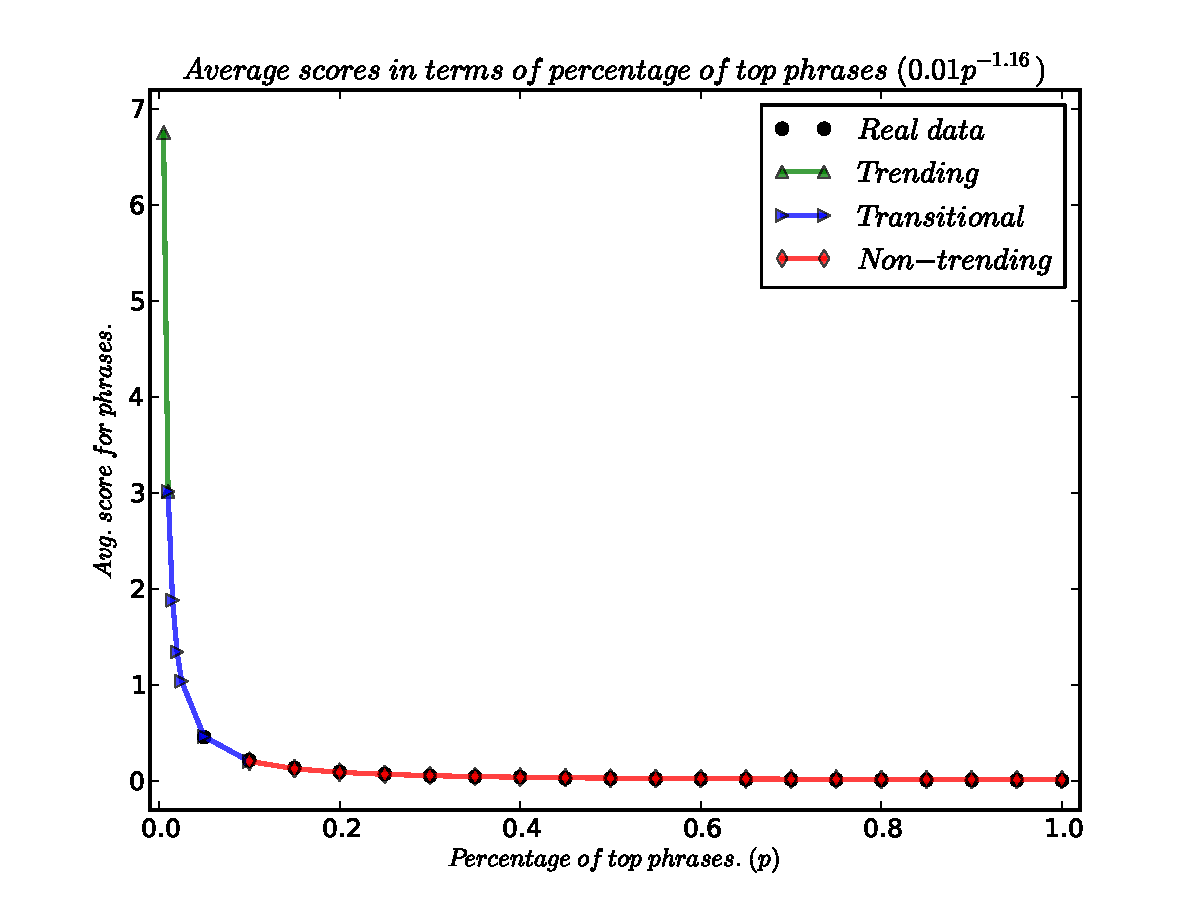
\includegraphics[width=2.2in]{images/par_est_PhraseScoresToReachXPercentage}}
%     \subfigure[Estimation of $S_t$]
%     {\label{fig:st}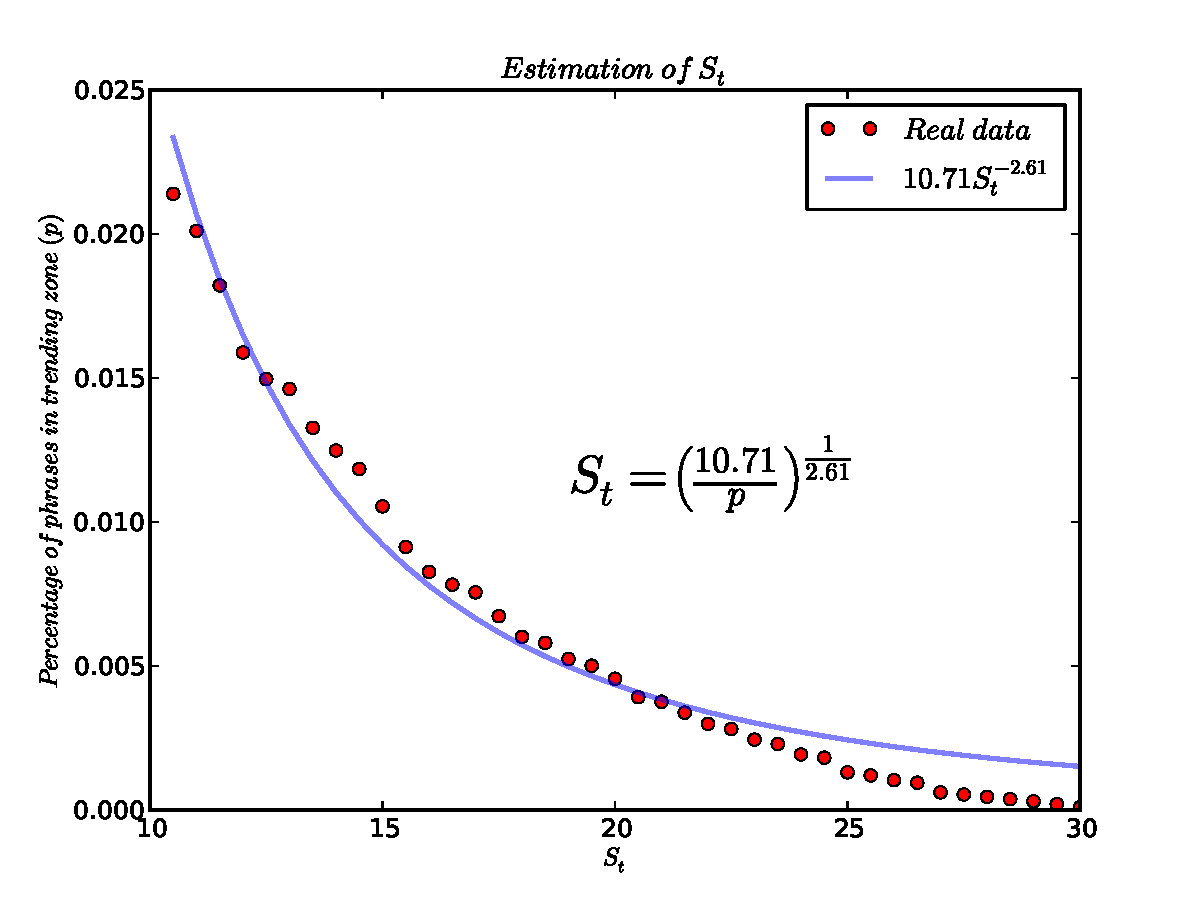
\includegraphics[width=2.2in]{images/par_est_DensitySt}}
%     \subfigure[Estimation of $S_p$]
%     {\label{fig:sp}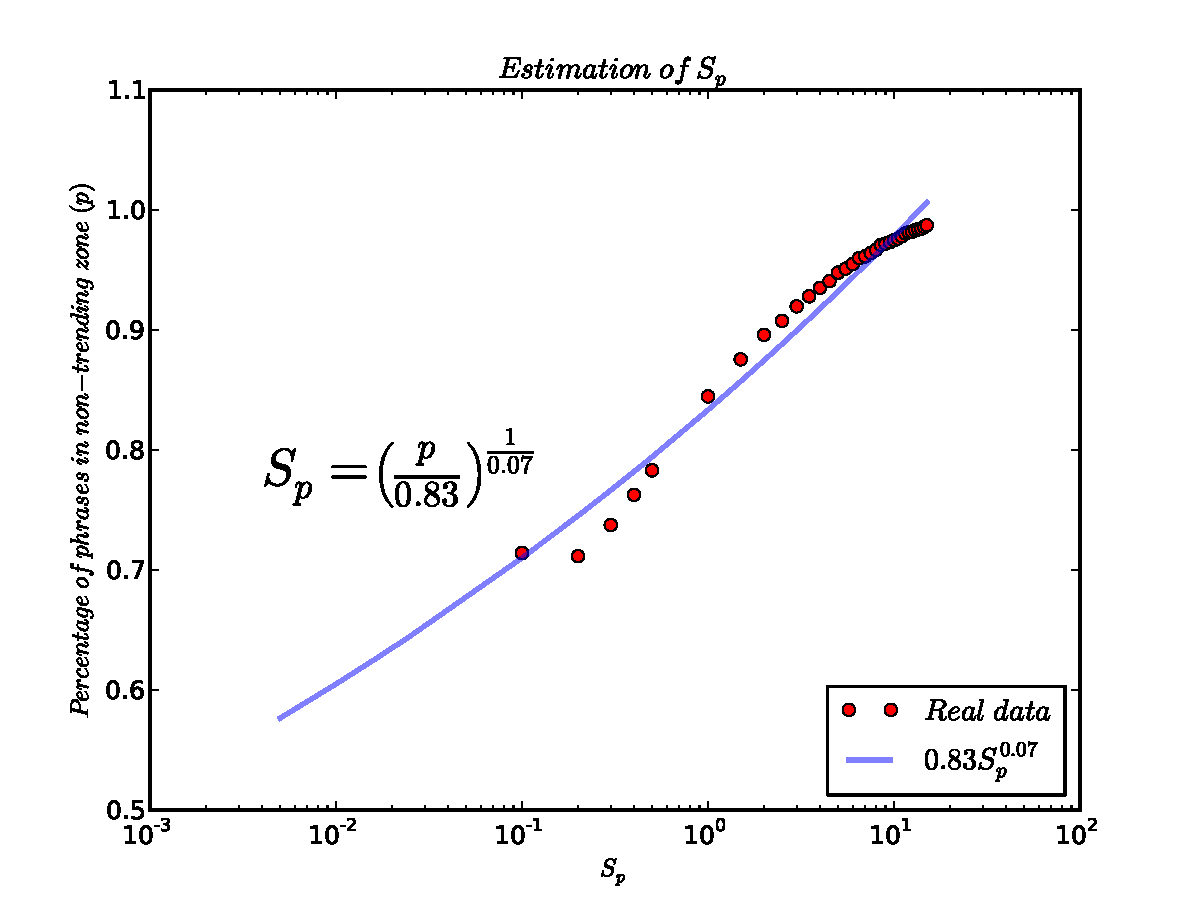
\includegraphics[width=2.2in]{images/par_est_DensitySp}}
%      \caption{Stream parameters estimation}
%   \label{fig:stream-parameters-1}
%   \end{center}
% \end{figure*}
% 
%To estimate the stream parameters we start by understanding the distribution of phrase scores. This analysis, helps us determine the distribution of phrases into the $3$ sets described in Section~\ref{sec:trend:discovery:problem} - trending, transitional and non-trending. We can then use this in determining the value of $S_t$ and $S_p$. We then use size of candidate phrase set $C_t$ as a metric to estimate maximum phrase inactivity time $T_{pi}$.
%
%\medskip\noindent\textbf{Phrase Score Distribution}: To understand the distribution of phrase scores, we process documents from the trending topic stream, updating the phrase scores using the equation Proposition~\ref{pro:candidate-phrase-score}. We set $\lambda_c = 0.80$ and process the stream for $2.5$ hours ($150$ minutes), noting down the phrase scores in $C_t$ every $5$ minutes. We then take these 30 sets of phrase scores and sort all of them to calcuate the average phrase scores at different levels of top phrases as shown in Figure~\ref{fig:phrase-by-percentage}. Based on this figure we can decide the split of phrases into different sets. Note that, the split of phrases is dependent on the application requirements. In this paper, we decided to use the following split- (i) Trending (green): Top $0.5\%$ phrases (ii) Transitional (blue): Middle $0.5-10\%$ phrases (iii) Non-trending (red): Bottom $90\%$.
% 
%\medskip\noindent\textbf{Estimation of $S_t$}: Like in previous case, to estimate the value of $S_t$, we process the documents from trending topic stream. During every $5$ minutes interval, we calculate the percentage of phrases above $\theta_{tt}$, calculated using the formula mentioned in Theorem~\ref{the:threshold}. We calculate $\theta_{tt}$ for different values of $S_t$. The values for $\eta$ and $C_t$ are obtained from the stream, and $\lambda_c = 0.80$. The variation of percentage of top phrases above $\theta_{tt}$ with $S_t$ is shown in Figure~\ref{fig:st}. Using this curve we get $S_t$ as a function of percentage of top phrases $p$.
%\begin{align*}
%S_t = \left(\frac{10.71}{p}\right)^{\frac{1}{2.61}}
%\end{align*}
%From analysis of phrase scores we decided to consider top $0.5\%$ phrases as trending. Hence, for $p=0.005$ we have $S_t=18.96$.
%
%\medskip\noindent\textbf{Estimation of $S_p$}: Similar to $S_t$, to calculate $S_p$, we process documents from trending topic stream. We use the formula in Theorem~\ref{the:threshold} to calculate $\theta_{pt}$ for different values of $S_p$. At every $5$ minutes interval, we calculate the percentage of phrases that are below $\theta_{pt}$. The variation of percentage of top phrases below $\theta_pt$ with $S_p$ is shown in Figure~\ref{fig:sp}. Using this curve we get $S_p$ as a function of percentage of top phrases $p$.
%\begin{align*}
%S_t = \left(\frac{p}{0.83}\right)^{\frac{1}{0.07}}
%\end{align*}
%Since, $90\%$ phrases are non-trending, for $p=0.9$, we have $S_p=3.02$.
%
%\begin{figure}[!t]
%\begin{center}
%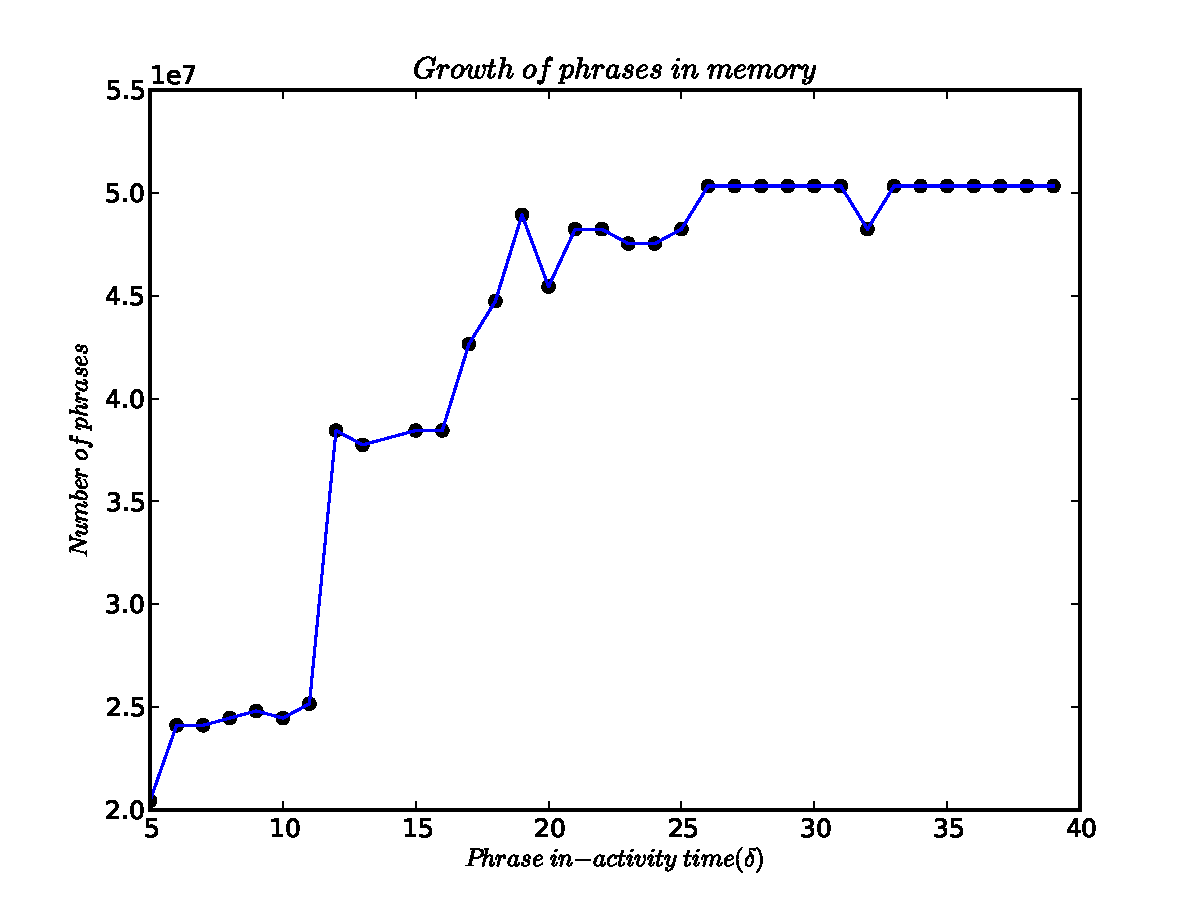
\includegraphics[width=3.0in]{images/par_est_PhraseInactivity}
%\caption{Estimation of $T_{pi}$}
%\label{fig:stream-parameters-2}
%\end{center}
%\end{figure}
%
%\medskip\noindent\textbf{Estimation of $T_{pi}$}: Ideally, we shouldn't have to prune $C_t$. But, for efficiency pruning it becomes necessary. If maximum phrase inactivity time $T_{pi}$ is very low, then the phrases are not allowed to trend, while if it is very high $C_t$ becomes very large. Hence, we determine the size of $C_t$ for increasing values of $T_{pi}$, and pick a value where $C_t$ is not very large and $T_{pi}$ is uniform. The variation of size of $C_t$ with increaseing $T_{pi}$ is shown in Figure~\ref{fig:stream-parameters-2}. Based on this, we set $T_{pi} = 7$ minutes.

%\subsection{Deterministic Vs Randomized Algorithm}
%\begin{figure}[!t]
%\begin{center}
%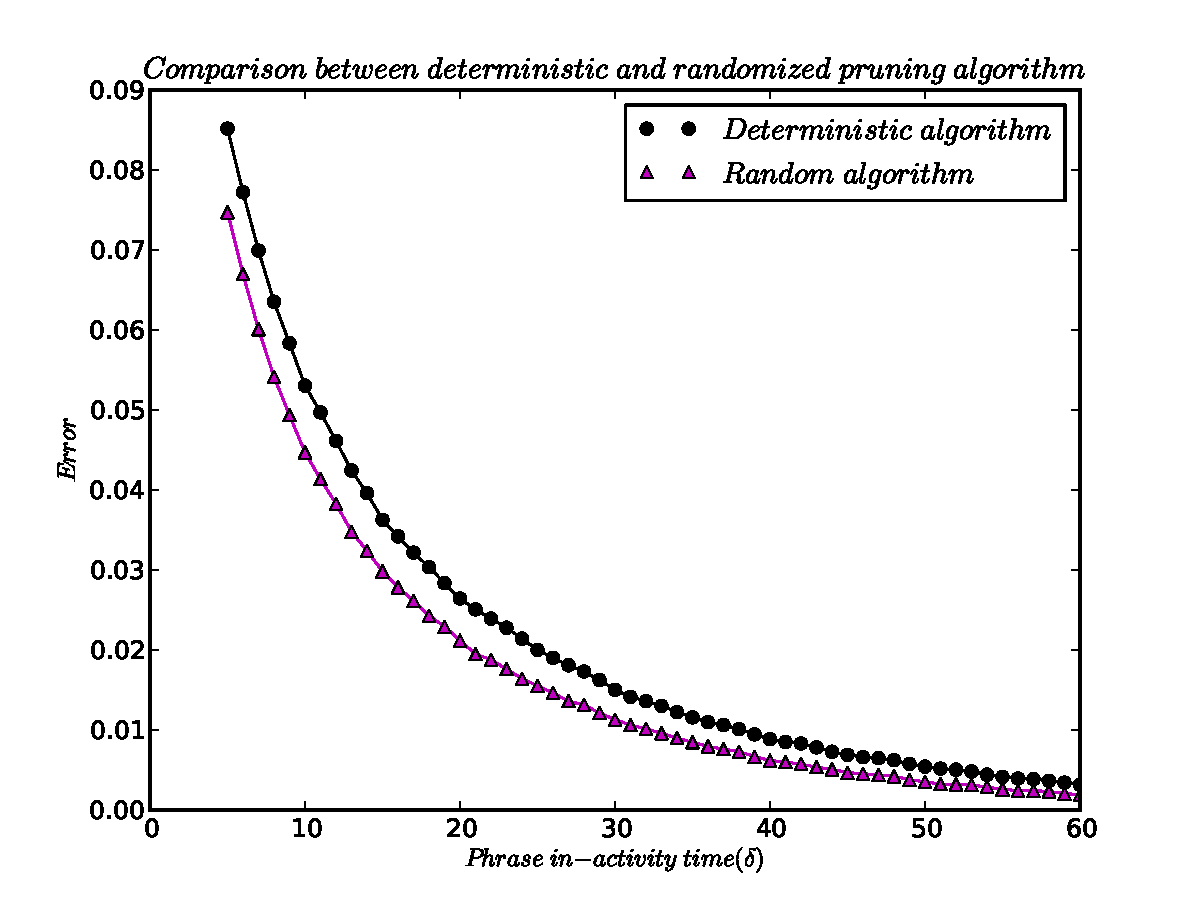
\includegraphics[width=3.0in]{images/par_est_PhraseInactivityComparison}
%\caption{Deterministic vs random}
%\label{fig:det-vs-random}
%\end{center}
%\end{figure}
%
%In Section~\ref{sec:trend:discovery:problem}, we described a deterministic and a randomized approach to prune $C_t$. We now compare these two different approaches using pruning error. Pruning error occurs when an algorithm marks a phrase to be pruned that is growing instead of decaying in the non-trending set. The performance of these two algorithms is shown in Figure~\ref{fig:det-vs-random}. As expected, the error decreases as $T_{pi}$ increases in both the cases, but this results in in-efficiency due to larger $C_t$. We also observe that magenta colored randomized algorithm performs better than the deterministic algorithm. Hence, in this paper we will be using randomized algorithm for pruning $C_t$.
%
%
%\subsection{Comparison with Sanderson's Approach}
% \begin{figure*}
%   \begin{center}
%     \subfigure[Running time]
%     {\label{fig:running}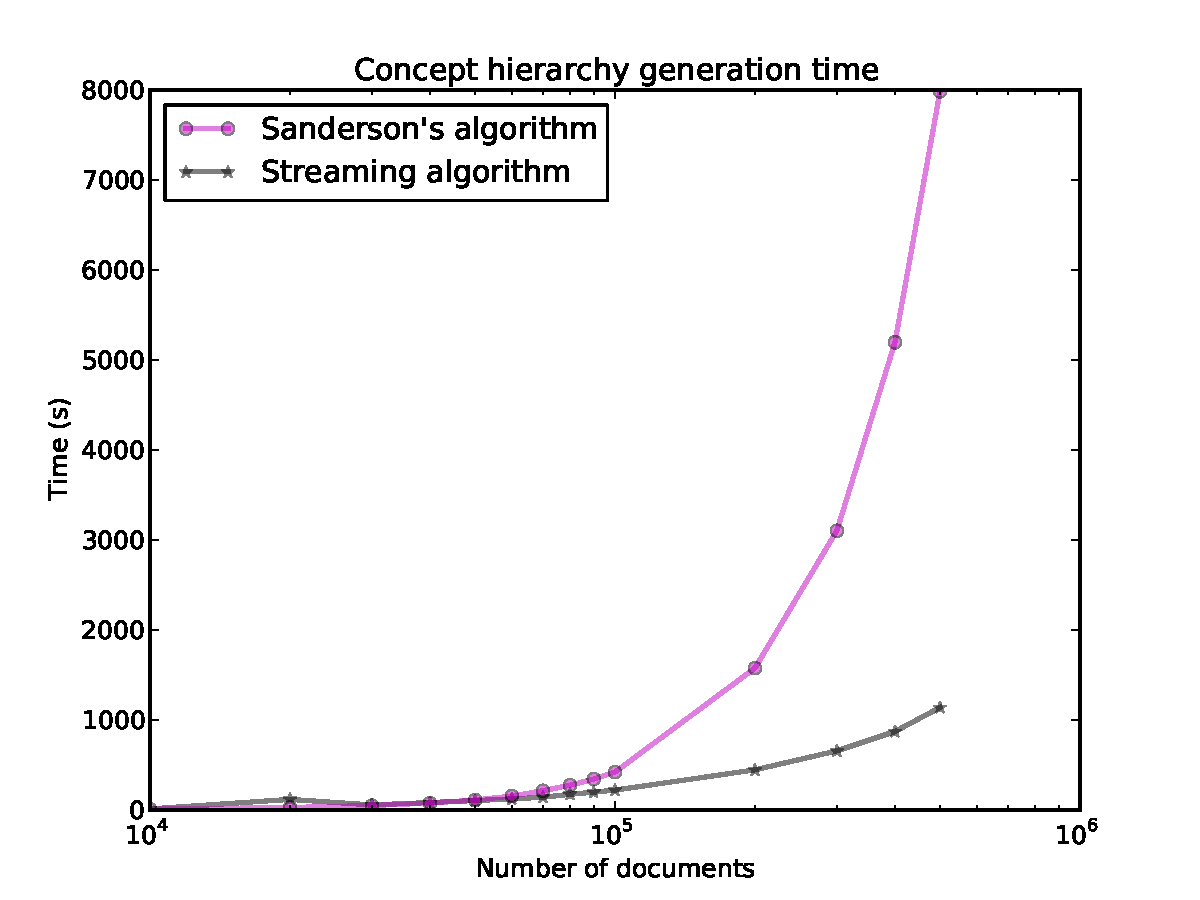
\includegraphics[width=3in]{images/experiments_concept_hierarchy_running_time}}
%     \subfigure[Topic Quality]
%     {\label{fig:quality}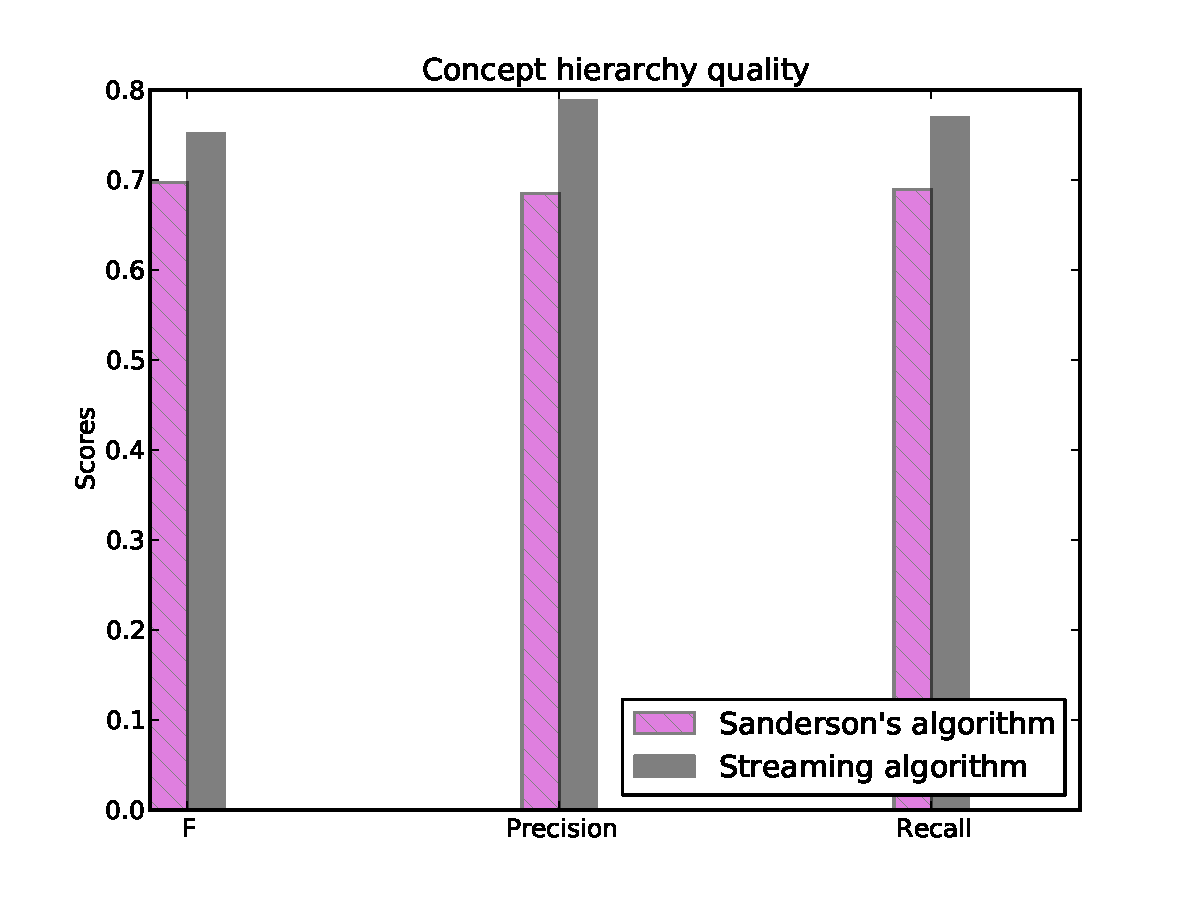
\includegraphics[width=3in]{images/experiments_concept_hierarchy_quality}}
%      \caption{Comparison with Sanderson's approach}
%   \label{fig:comaprison-sanderson}
%   \end{center}
% \end{figure*}
%
%We now compare the performance of our algorithm to discover phrase topic hierarchies with that of a popular approach to determine concept hierarchies suggested by Sanderson and Croft \cite{Sanderson:1999:derivingconcept}. 
%
%In \cite{Sanderson:1999:derivingconcept} , Sanderson and Croft, present a approach to generate concept hierarchies from text documents, based on the principle of subsumption. A term $x$ is said to subsume another term $y$, if $x$ describes a concept that is more general than a concept described by $y$. If $x$ subsumes $y$, then $x$ is the parent of $y$ in the concept hierarchy tree. They use co-occurrence information from a text document set, to derive the relationship between $x$ and $y$. They first present conditions to determine if a term $x$ has subsumed $y$, and then relax these conditions to increase the number of relationships discovered. In the relaxed version, $x$ subsumes $y$, if both the following conditions are satisfied:
%\begin{align*}
%P(x|y) \geq 0.8 \text{ and } P(y|x) < 1
%\end{align*}
%\noindent where, the value 0.8 is not fixed, but dependent on the application for which concepts are being generated.
%
%To compare our approach to discover phrase topic hierarchy with Sanderson's algorithm, we used the domain specific stream discussed in Section~\ref{sec:data-stream}. We first estimated the parameters for domain specific streams as shown before. To do this, we set $\lambda_c=0.80$ and consider top $1\%$ of phrases as trending. We then, generated concept hierarchies using both these approaches and compared the performance of the algorithms.
%
%\medskip\noindent\textbf{Running Time Comparison}: The comparison of running times for Sanderson's and our algorithm is shown in Figure~\ref{fig:running}. We observe that the time taken for construction of concept hierarchy increases at higher rate using Sanderson's algorithm compared to our algorithm. The reasons for this increase in running time is because, detection of concept hierarchies in Sanderson's algorithm involves performing ${{n}\choose{2}}$ comparisons for $n$ phrases. Hence, as the number of documents increase $n$ increases accordingly. In our approach, since we select phrases based on their score, the running time is not directly dependent on the number of documents and hence we see an improved performance.
%
%\medskip\noindent\textbf{Concept Hierarchy Quality Comparison}: Determining the quality of concept hierarchies generated by the algorithms is not trivial. Conducting user studies is a popular approach that has been used to determine quality. But, the number of concept trees in phrase topic hierarchies, generated from data streams, is large and this makes conducting good user studies impractical. Hence, we use an indirect method to determine the quality of hierarchies generated by these two algorithms. 
%
%Like described before, phrase topic hierarchies is composed of a set of disconnected DAGs, where every DAG describes some topic. For example, we might have a DAG for Middle-East, another one for Super Bowl, etc. Since, we used domain specific stream to generate phrase topic hierarchies, ideally every node in a particular DAG should belong to a single domain. For example, given a domain like sports, a DAG describing Super Bowl should contain nodes related to sports only. We can use this information to determine the `purity' of generated topic hierarchies. 
%
%We use precision, recall and F-measure as metrics to determine quality of topic hierarchies. The performance of the two algorithms is shown in Figure~\ref{fig:quality}. We see that the quality of concepts generated by our algorithm is close to that generated by Sanderson's algorithm.
%
%\subsection{Examples of Topic Hierarchies}
% \begin{figure*}[ht]
%   \begin{center}
%     \subfigure[Real hierarchy.]
%     {\label{fig:concept-hierarchies-super-bowl-real}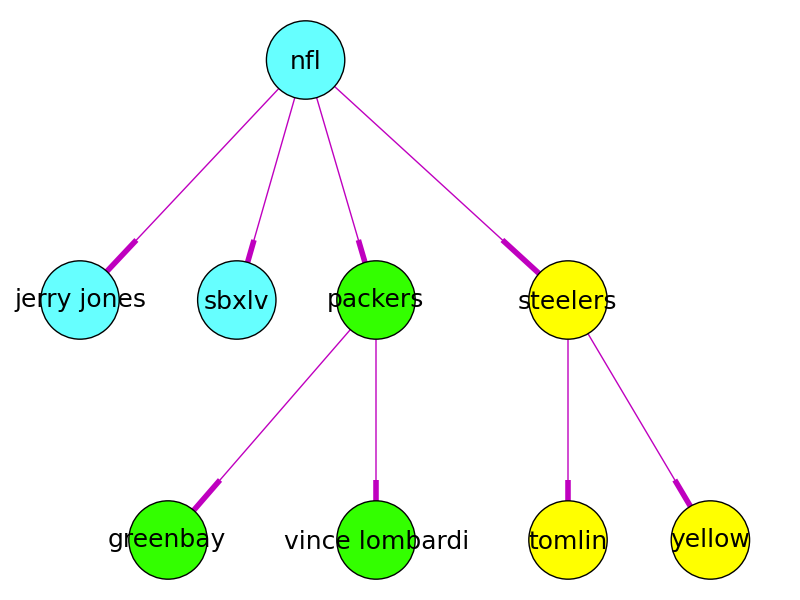
\includegraphics[width=2.2in]{images/superbowlReal}}
%     \subfigure[Driven by generality.]
%     {\label{fig:concept-hierarchies-super-bowl-general}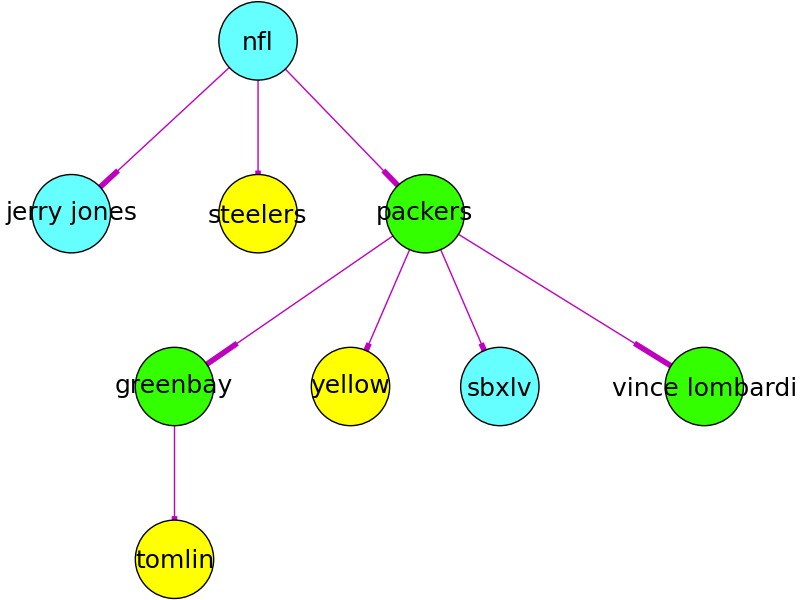
\includegraphics[width=2.2in]{images/superbowlDegree}}
%     \subfigure[Driven by popularity.]
%     {\label{fig:concept-hierarchies-super-bowl-popular}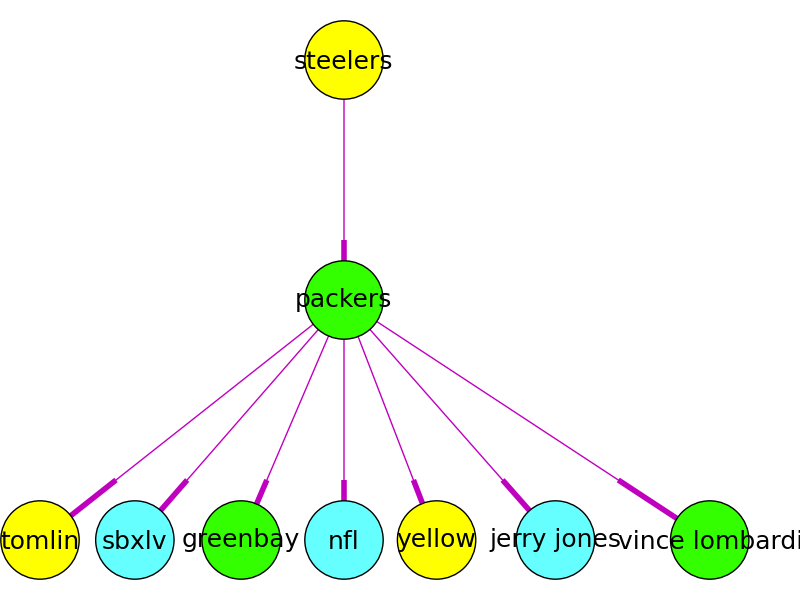
\includegraphics[width=2.2in]{images/superbowlNodeWeight}}
%      \caption{Concept hierarchies during Super Bowl, 2011 between Green Bay Packers and Pittsburgh Steelers.}
%   \label{fig:concept-hierarchies-super-bowl}
%   \end{center}
% \end{figure*}
% 
%\medskip\noindent\textbf{Comparison of Topic Hierarchy Metrics}: In Section~\ref{sec:phrase-topic-hierarchy}, we described two metrics that can be used to generate phrase topic hierarchies, depending on the type of information we are interested in. In Figure~\ref{fig:concept-hierarchies-super-bowl}, we show the example of topic hierarchy generated for Super Bowl that was played between Green Bay Packers and Pittsburgh Steelers on February $6^{th}$, 2011. The hierarchy was generated using trending topic stream and for 6 hours of data prior to the kick-off.
%
%We first classified the phrases in Super Bowl cluster into 3 categories: packers (green), steelers (yellow) and neutrals (cyan). We then picked 3 phrases from each category and compared the topic hierarchy generated using each of the hierarchy metrics. The manually constructed concept hierarchy, for the selected keywords, based on our understanding of these categories is shown in is shown in Figure~\ref{fig:concept-hierarchies-super-bowl-real}. The hierarchies driven by generality and popularity are shown in Figure~\ref{fig:concept-hierarchies-super-bowl-general} and Figure~\ref{fig:concept-hierarchies-super-bowl-popular} respectively. To compare the hierarchies, generated using metrics, with the manually constructed hierarchy, we convert DAG to a tree by keeping only the edge with maximum weight. Hence, in Figure~\ref{fig:concept-hierarchies-super-bowl-popular}, though vertices like ``steelers'' drive other vertices in the graph, the extra edges are not shown.
%
%We observe that the hierarchy generated by generality is very similar to the manually constructed hierarchy, while the hierarchy generated by popularity is very different from the real hierarchy. This is expected because, whenever an event (sporting events, product launch, etc.) occurs, the phrases that detail the event like people making news, product names, etc., trend and these phrases drive the event in social media, while other phrases like championship the game is played in, company name, etc, get associated with several phrases but don't actually trend. Hence, in our case, the teams participating in Super Bowl are driving the cluster prior to the start of the game while phrases like ``nfl'' are associated with all the phrases but not trending higher than other key phrases.
%
%In this way, depending upon the requirements of the application, we can use any of these metrics to generate specific hierarchies. 
%
%\begin{table*}[ht] 
%\begin{center}
%\begin{tabular}{c|c|p{10cm}}
%\hline
%\textbf{Day} & \textbf{Time interval length} & \hspace{2cm} \textbf{Concepts Driven by ``Middle East''}\\ \hline \hline
%5 Feb, 2011 04:13:00 CST &  & Tahrir Square, Hosni Mubarak, Vice President, Crisis\\ 
%5 Feb, 2011 10:43:00 CST & 1 hour & Impact, Egypt, Protests, jan25, Perfect Storm, Hilary Clinton warns\\
%5 Feb, 2011 16:08:00 CST &  & Israel\\ 
%\hline
%5 Feb, 2011 00:33:00 CST &  & Al-Jazeera, America, Protesters, Shockwaves\\ 
%5 Feb, 2011 06:38:00 CST &  & USA, Egypt-Israel, Terror\\ 
%5 Feb, 2011 12:43:00 CST & 6 hours & Impact, Hillary Clinton, Anti-Government, Perfect Storm, Middle-East Talks,  Mideast Quartet\\ 
%5 Feb, 2011 18:28:00 CST &  & Perfect Storm, Rulers, Anti-Government, Sentiments, Hilary Clinton warns, Meydan, Gen. Hasan Rawini\\ 
%\hline
%5 Feb, 2011 00:00:00 CST &  24 hours & Hilary Clinton, Rulers, Perfect Storm\\ 
%\hline
%7 Feb, 2011 00:00:00 CST & 7 days  & Yemen, Ahmed Ezz, Tony Blair, Facebook, BBC Question time, Iran Election, Transition, Force, Glenn, Violence, BBC Question time, Fears, Riots \\ 
%\hline
%15 Feb, 2011 00:00:00 CST &  14 days & Syria, Yemen, Sudan, Trepidation, Riots, BBC Question time, Mehdi, Glenn, Mark Zuckerberg\\ 
%\hline
%\end{tabular}
%\end{center}
%\caption{Concepts driven by ``Middle East'' at different time intervals.}
%\label{table:middle-east-time-interval}
%\end{table*}
%
%\medskip\noindent\textbf{Variation of Concepts With Time}: An example of how concepts that are being driven by a phrase change at different time interval is shown in Table~\ref{table:middle-east-time-interval}. We used trending topic stream and observed the phrases Middle-East was driving during a 15-days interval in February, 2011. We used popularity metric to determine the driven phrases.
%
%During time intervals of 1 hour we see key phrases being driven like ``Tahrir Square'', ``jan25'' etc. Moving to a bigger window of 6 hours we see still a lot of key words like those that were observed at 1 hour. But, at larger windows like 7 and 14 days we don't see specific event related phrases but general phrases like countries effected by the uprisings, general happenings like riots, violence etc., being driven.







{\scriptsize
 \bibliographystyle{abbrv}
 \bibliography{sigproc}
}
\balancecolumns % GM July 2000

\end{document}
